\chapter{Diseño dinámico}
\label{cap:disenoDinamico}

Este capítulo presenta el comportamiento dinámico del sistema en tiempo de ejecución. Se detalla el flujo de interacciones del caso de uso de inicio de sesión (\textbf{CU Login}) mediante un diagrama de secuencia embebido en TikZ y se describe el comportamiento ante diferentes escenarios.

%---------------------------------------------------------
\section{Diseño dinámico del CU login}
\label{sec:disenoDinamicoLogin}

El inicio de sesión permite autenticar de forma segura a los colaboradores y direccionar sus permisos según su rol. El diagrama de secuencia UML describe el paso de mensajes entre los componentes del sistema:

\begin{figure}[htbp!]
\centering
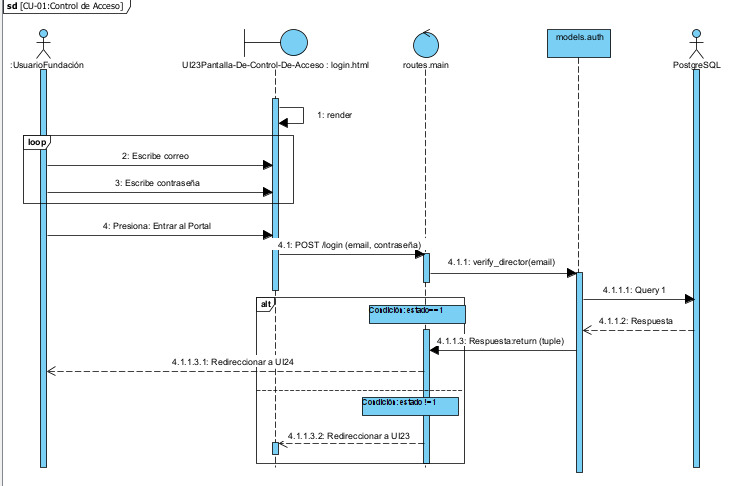
\includegraphics[width=0.85\textwidth]{CU/CU1.jpeg}
\caption{Diagrama de secuencia dinámico para el Caso de Uso de Inicio de Sesión (Login).}
\label{fig:secuenciaLogin}
\end{figure}

\subsection{Descripción de las Interacciones}
\begin{enumerate}
    \item El usuario introduce sus credenciales (correo electrónico y contraseña) en la interfaz del navegador y hace clic en el botón \textit{Ingresar}. Esto genera una petición HTTP de tipo \texttt{POST} dirigida al endpoint \texttt{/login} del controlador de la aplicación.
    \item El controlador (\texttt{routes.main}) intercepta la petición y llama de forma secuencial a las funciones de validación del modelo de autenticación (\texttt{models.auth.verify\_director} y, en caso de fallar, \texttt{models.auth.verify\_coordinador}).
    \item El modelo abre un cursor de base de datos a través de la función \texttt{get\_db\_cursor} y ejecuta una consulta SQL parametrizada a PostgreSQL, buscando el registro del personal mediante su correo registrado.
    \item El servidor PostgreSQL procesa la consulta y retorna los datos correspondientes: la clave CURP del personal, su nombre, el \textit{hash} de la contraseña cifrada y el estado actual de su cuenta de acceso.
    \item El modelo propaga el resultado al controlador en forma de tupla o \texttt{None} si el correo no existe.
    \item El controlador ejecuta localmente la validación del estado (debe ser un usuario habilitado) y valida la coincidencia de la contraseña ingresada con el hash cifrado almacenado utilizando la librería de seguridad.
    \item Si la validación es correcta, el controlador crea las variables de sesión del usuario en la cookie y responde con una redirección HTTP \texttt{302} hacia el panel correspondiente a su rol (Director o Coordinador). En caso de error, retorna el control al login desplegando una alerta visual (mensaje de error en pantalla).
\end{enumerate}

%---------------------------------------------------------
\section{Diseño dinámico del CU-02: Gestión de usuarios y roles}
\label{sec:disenoDinamicoCU02}

Permite al Director registrar, editar, inhabilitar y eliminar cuentas de usuarios de los profesionales en el sistema.

\begin{figure}[htbp!]
\centering
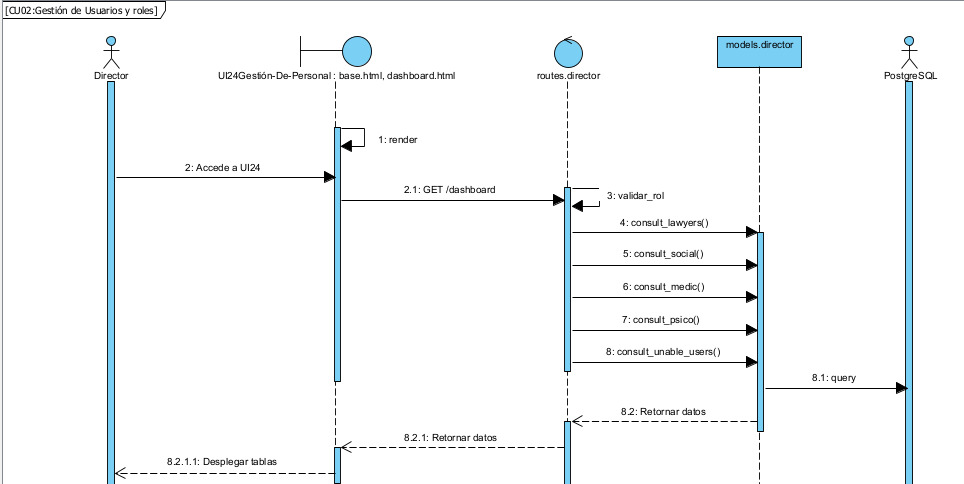
\includegraphics[width=0.85\textwidth]{CU/CU2.jpeg}
\caption{Diagrama de secuencia para el Caso de Uso de Gestión de usuarios y roles.}
\label{fig:secuenciaCU02}
\end{figure}

\subsection{Descripción de las Interacciones}
El Director ingresa al formulario de registro en la interfaz de usuario. Al guardar, se envía una petición POST al controlador \texttt{routes.director.registrar}, que valida los datos obligatorios y la unicidad del CURP/RFC, llamando al modelo \texttt{models.director.user\_register} para insertar el registro en la base de datos PostgreSQL.

%---------------------------------------------------------
\section{Diseño dinámico del CU-03: Gestión de expediente del NNA}
\label{sec:disenoDinamicoCU03}

Permite la creación, actualización y consulta del Expediente Único (FUD) de un menor.

\begin{figure}[htbp!]
\centering
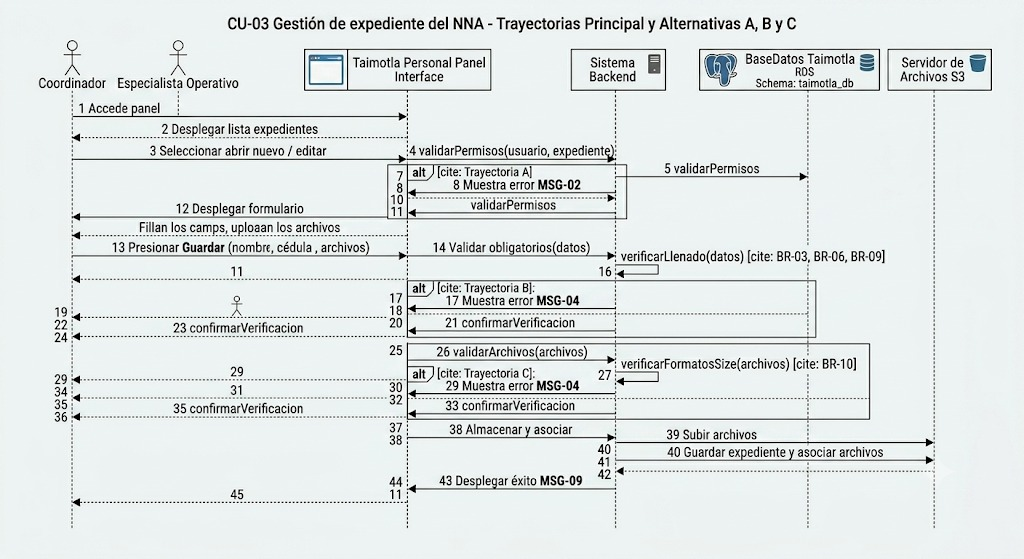
\includegraphics[width=0.85\textwidth]{CU/CU3.jpeg}
\caption{Diagrama de secuencia para el Caso de Uso de Gestión de expediente del NNA.}
\label{fig:secuenciaCU03}
\end{figure}

\subsection{Descripción de las Interacciones}
El Trabajador Social captura los datos del menor en las pestañas del expediente único. Al guardar, el controlador \texttt{routes.director.guardar\_expediente} invoca a \texttt{models.nna.guardar\_nna\_db}. El modelo realiza inserciones o actualizaciones en las tablas \texttt{domicilio}, \texttt{personas\_expediente}, \texttt{nna}, \texttt{hecho\_victimal} y \texttt{entorno\_familiar} agrupadas en una única transacción de base de datos para mantener la consistencia.

%---------------------------------------------------------
\section{Diseño dinámico del CU-04: Asignación de casos}
\label{sec:disenoDinamicoCU04}

Permite al Director asignar un expediente único a un equipo multidisciplinario específico para su seguimiento.

\begin{figure}[htbp!]
\centering
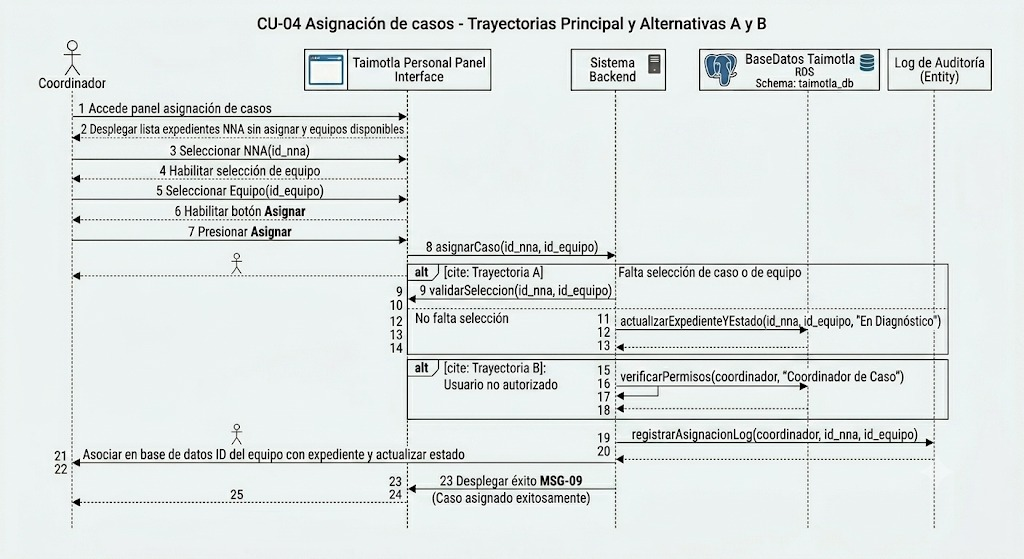
\includegraphics[width=0.85\textwidth]{CU/CU4.jpeg}
\caption{Diagrama de secuencia para el Caso de Uso de Asignación de casos.}
\label{fig:secuenciaCU04}
\end{figure}

\subsection{Descripción de las Interacciones}
El Director selecciona el expediente y el equipo de trabajo en la interfaz. El controlador envía los datos al modelo de persistencia para asociar el identificador del equipo en el registro correspondiente de la tabla \texttt{expediente}.

%---------------------------------------------------------
\section{Diseño dinámico del CU-05: Crear equipo de trabajo}
\label{sec:disenoDinamicoCU05}

Permite al Director crear un nuevo grupo multidisciplinario de profesionales designando a un Coordinador y entre 2 y 4 especialistas de diferentes áreas.

\begin{figure}[htbp!]
\centering
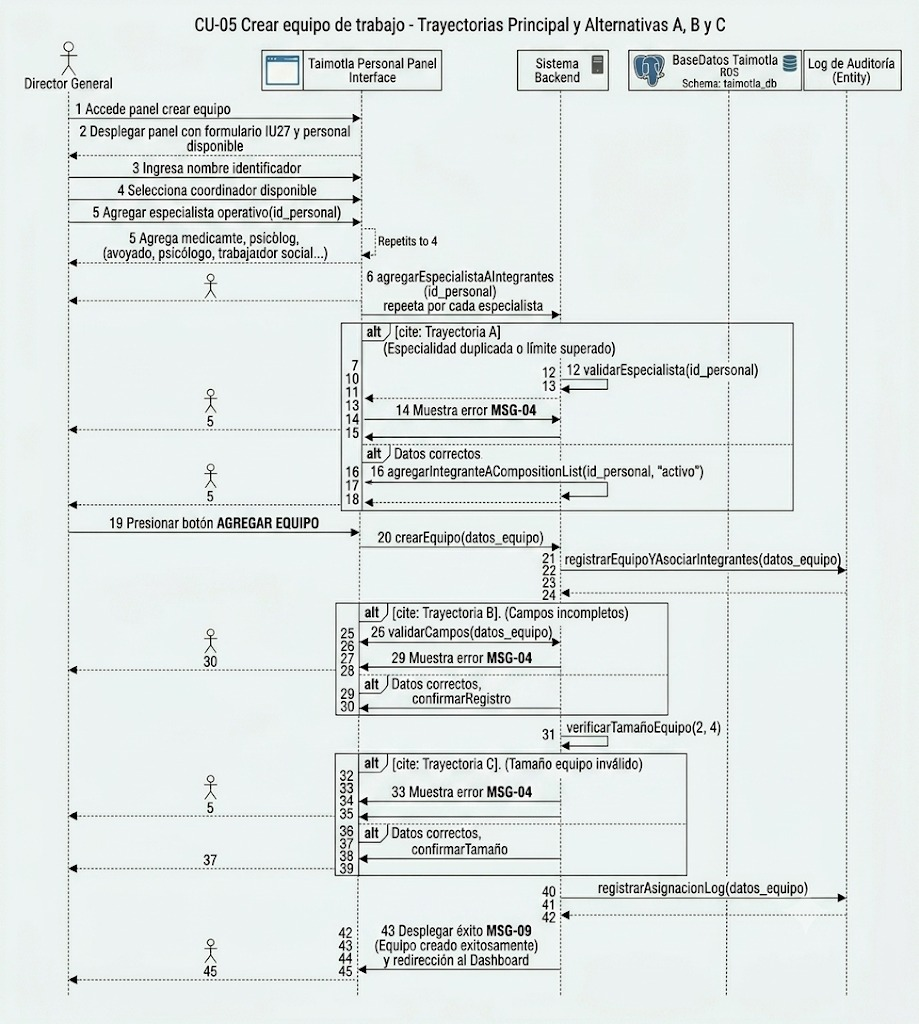
\includegraphics[width=0.85\textwidth]{CU/CU5.jpeg}
\caption{Diagrama de secuencia para el Caso de Uso de Crear equipo de trabajo.}
\label{fig:secuenciaCU05}
\end{figure}

\subsection{Descripción de las Interacciones}
El Director selecciona el coordinador y los miembros en el formulario. Al presionar guardar, el controlador \texttt{routes.director.crear\_equipo} valida el tamaño del equipo e invoca a \texttt{models.equipo.create\_team}, el cual crea el registro del equipo en la tabla \texttt{equipo} y registra a sus integrantes en la tabla \texttt{composicion\_equipo} de manera atómica.

%---------------------------------------------------------
\section{Diseño dinámico del CU-06: Gestionar equipos de trabajo}
\label{sec:disenoDinamicoCU06}

Permite al Director modificar la estructura o disolver los equipos de trabajo activos.

\begin{figure}[htbp!]
\centering
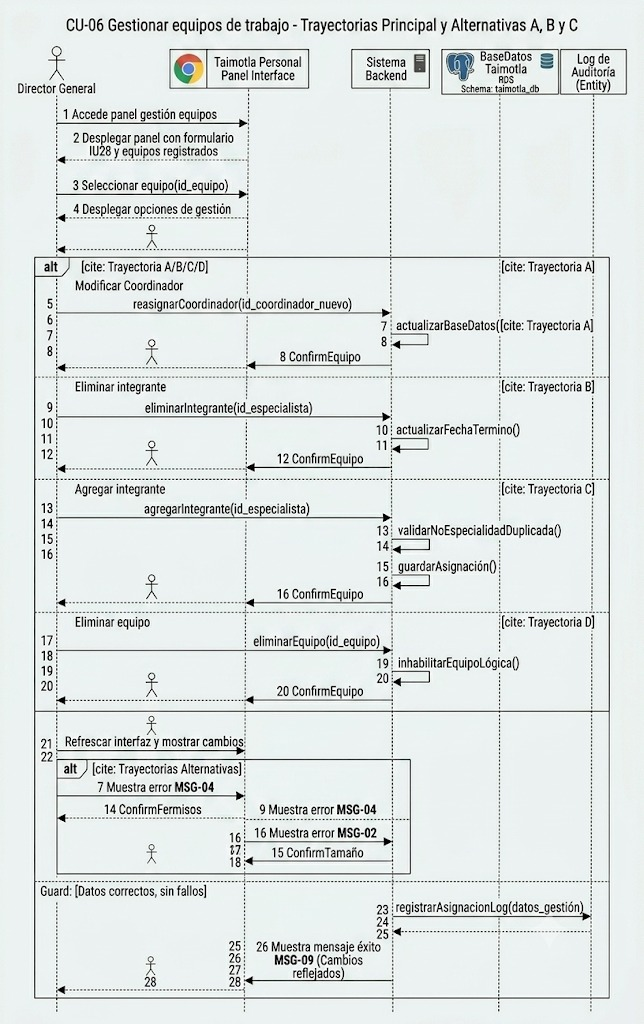
\includegraphics[width=0.75\textwidth]{CU/CU6.jpeg}
\caption{Diagrama de secuencia para el Caso de Uso de Gestionar equipos de trabajo (Disolución).}
\label{fig:secuenciaCU06}
\end{figure}

\begin{figure}[htbp!]
\centering
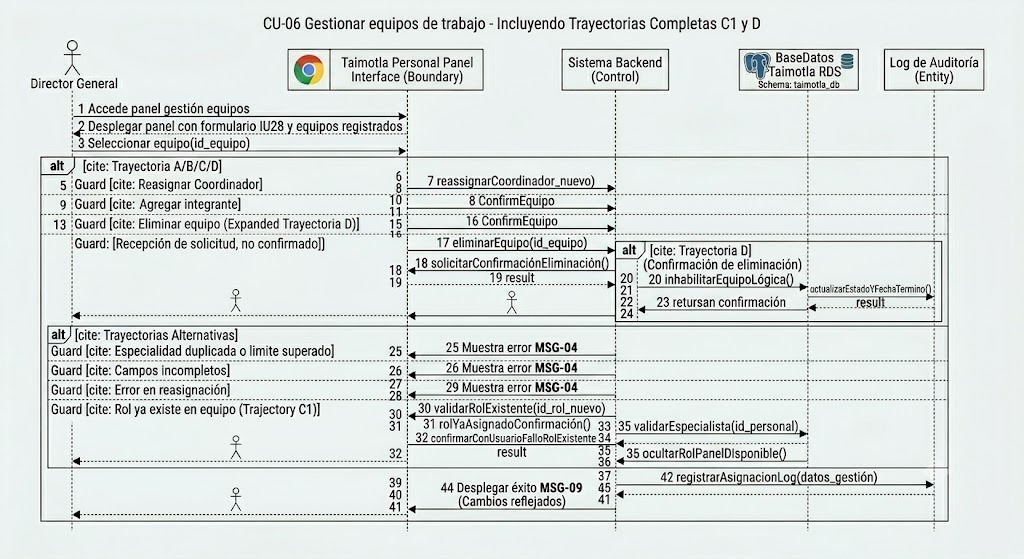
\includegraphics[width=0.85\textwidth]{CU/CU6_alternativas_c1_y_D.jpeg}
\caption{Diagrama de secuencia para el Caso de Uso de Gestionar equipos de trabajo (Adición/Remoción de Miembros).}
\label{fig:secuenciaCU06Alt}
\end{figure}

\subsection{Descripción de las Interacciones}
El Director puede reasignar el coordinador del equipo, agregar un nuevo integrante disponible o eliminar a un integrante cerrando su participación con la fecha de fin actual en la tabla \texttt{composicion\_equipo}. Para la disolución de un equipo, se actualiza su estado a inactivo y se cierran las asignaciones activas de todos los miembros.

%---------------------------------------------------------
\section{Diseño dinámico del CU-07: Consultar perfil y datos de cuenta}
\label{sec:disenoDinamicoCU07}

Permite a cualquier usuario autenticado visualizar su información personal, laboral y de contacto.

\begin{figure}[htbp!]
\centering
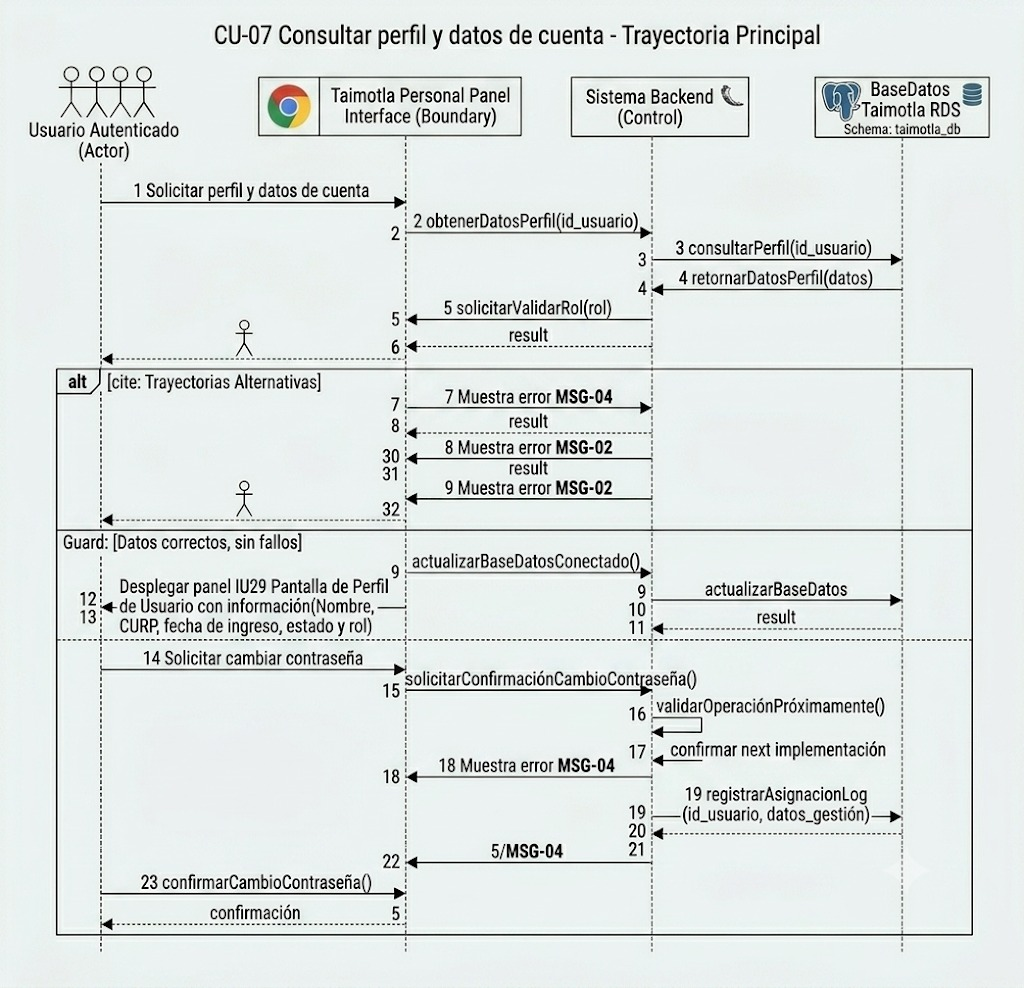
\includegraphics[width=0.85\textwidth]{CU/CU7.jpeg}
\caption{Diagrama de secuencia para el Caso de Uso de Consultar perfil y datos de cuenta.}
\label{fig:secuenciaCU07}
\end{figure}

\subsection{Descripción de las Interacciones}
Al presionar la opción en el menú, el controlador extrae la CURP de la sesión del usuario, realiza la consulta correspondiente de la información de su perfil utilizando las funciones del modelo y despliega la vista con los datos personales, de contacto y estatus laboral de la persona.

%---------------------------------------------------------
\section{Diseño dinámico del CU-08: Capturar valoración del Especialista}
\label{sec:disenoDinamicoCU08}

Permite a los Especialistas (Médicos, Abogados, Psicólogos) capturar y registrar sus valoraciones específicas del menor en el expediente.

\begin{figure}[htbp!]
\centering
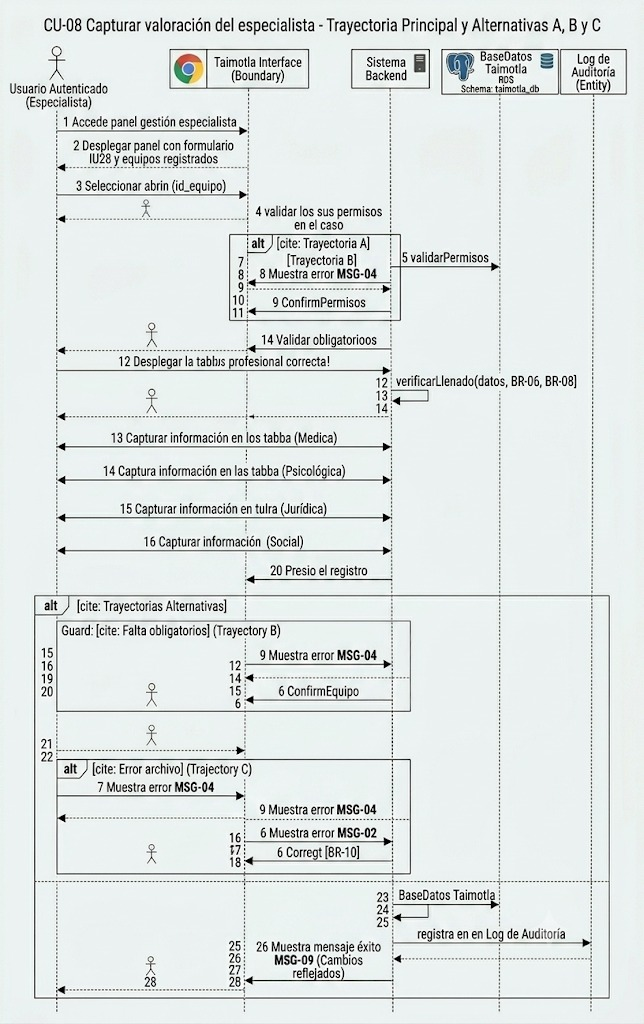
\includegraphics[width=0.75\textwidth]{CU/CU8.jpeg}
\caption{Diagrama de secuencia para el Caso de Uso de Capturar valoración del Especialista.}
\label{fig:secuenciaCU08}
\end{figure}

\subsection{Descripción de las Interacciones}
El Especialista ingresa a la pestaña correspondiente a su área del expediente, escribe las observaciones y valoraciones en el formulario, y al guardar se realiza un POST al servidor que valida y persiste las valoraciones específicas del menor.

%---------------------------------------------------------
\section{Diseño dinámico del CU-09: Gestión de personal por Coordinador}
\label{sec:disenoDinamicoCU09}

Permite al Coordinador del equipo consultar y reasignar tareas a los especialistas asignados a los casos bajo su jurisdicción.

\begin{figure}[htbp!]
\centering
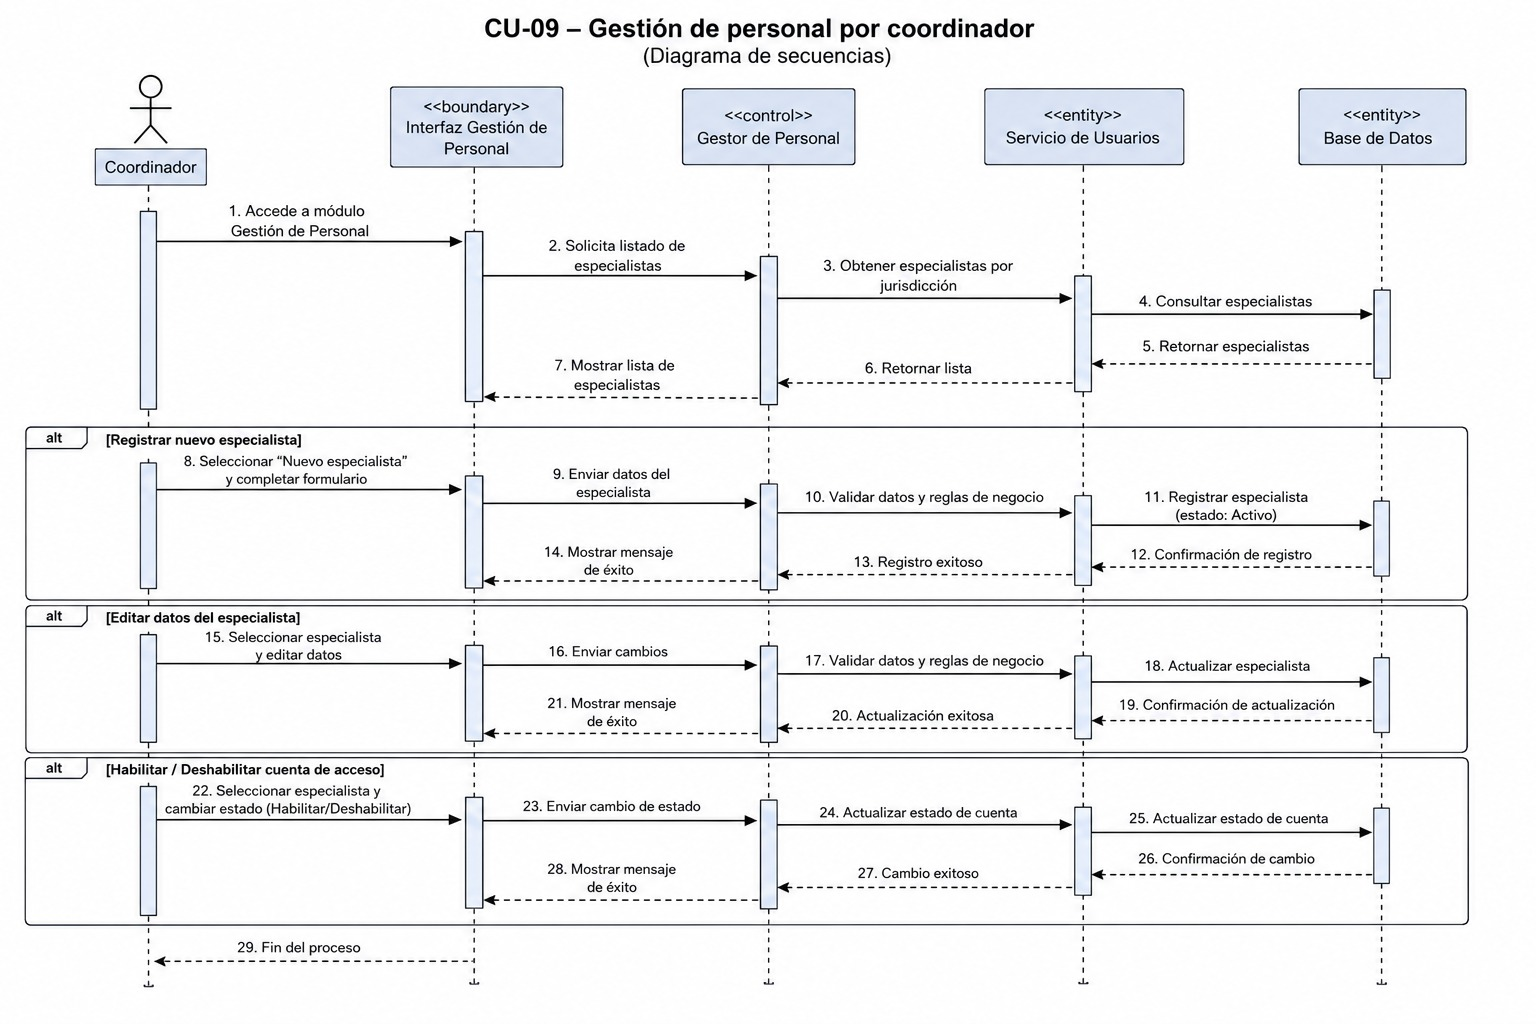
\includegraphics[width=0.85\textwidth]{CU/CU9.jpeg}
\caption{Diagrama de secuencia para el Caso de Uso de Gestión de personal por Coordinador.}
\label{fig:secuenciaCU09}
\end{figure}

\subsection{Descripción de las Interacciones}
El Coordinador accede a su panel de gestión y el sistema recupera la lista del personal a su cargo y los expedientes que tiene asignados, permitiendo modificar las asignaciones o monitorear los avances de las valoraciones de cada área.

%---------------------------------------------------------
\section{Diseño dinámico del CU-10: Registrar hecho victimal}
\label{sec:disenoDinamicoCU10}

Permite al Abogado registrar el reporte de hechos y los delitos detectados de los que el menor fue víctima.

\begin{figure}[htbp!]
\centering
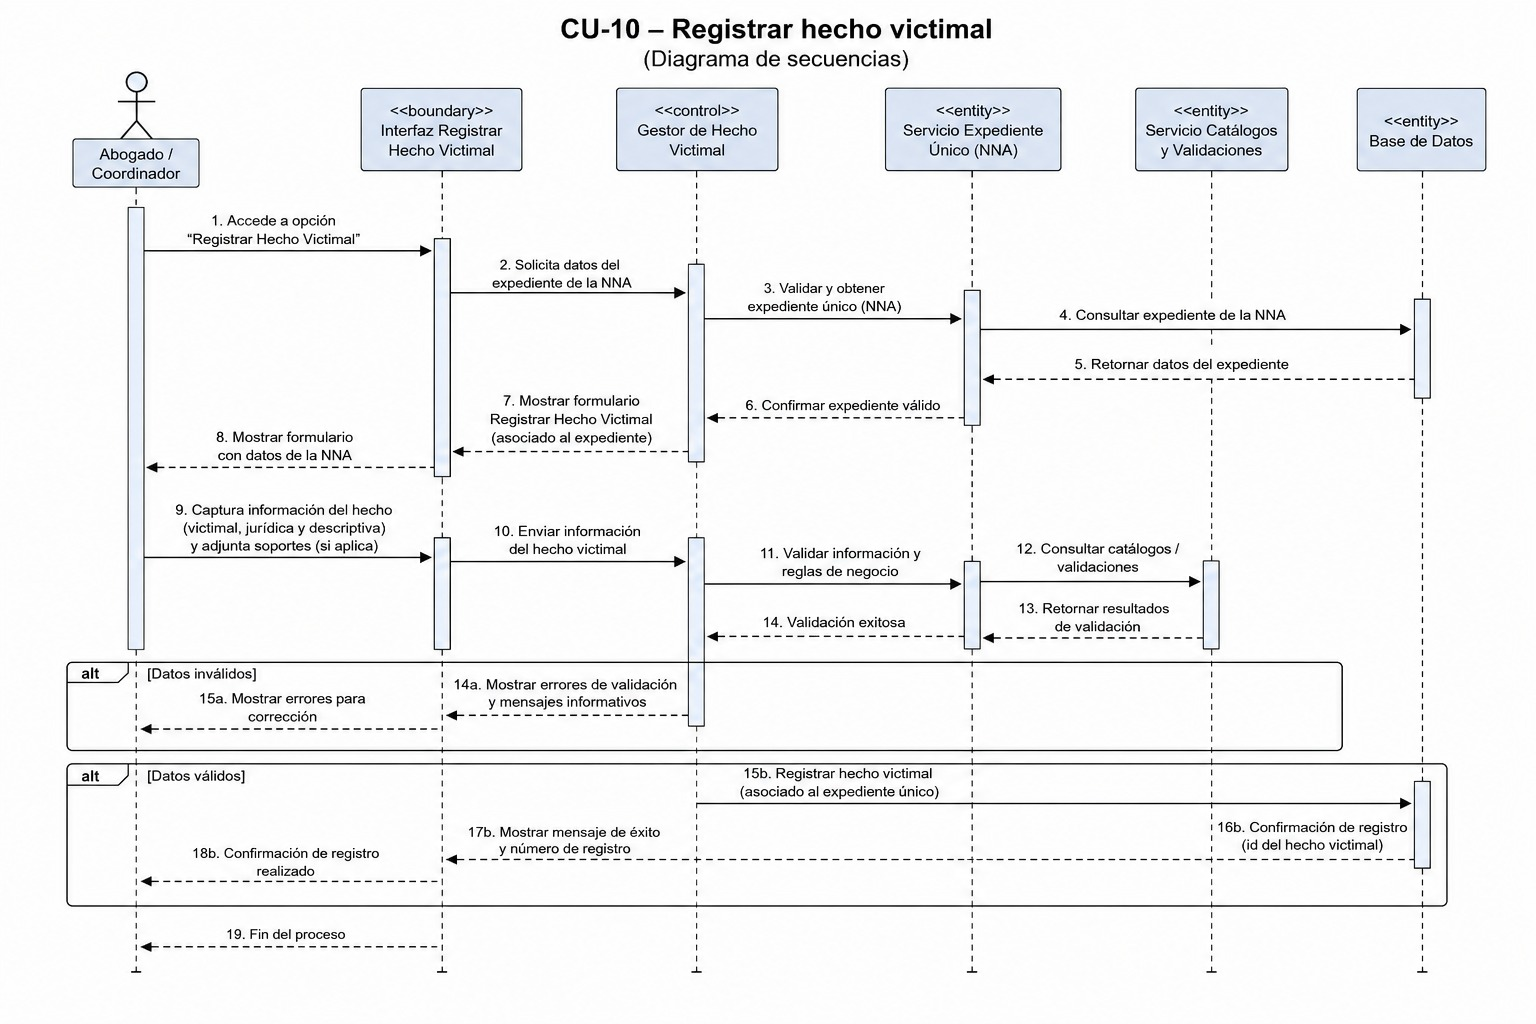
\includegraphics[width=0.85\textwidth]{CU/CU10.jpeg}
\caption{Diagrama de secuencia para el Caso de Uso de Registrar hecho victimal.}
\label{fig:secuenciaCU10}
\end{figure}

\subsection{Descripción de las Interacciones}
El Abogado ingresa al apartado correspondiente en la edición del expediente único, registra el número de reporte del caso, fecha de detención, delito y narración de hechos, y los envía al controlador, el cual realiza una inserción o actualización de la información en la tabla \texttt{hecho\_victimal} a través de la función de base de datos.

%---------------------------------------------------------
\section{Diseño dinámico del CU-11: Registrar Cuidador / Tutor}
\label{sec:disenoDinamicoCU11}

Permite al Trabajador Social capturar e integrar la información del cuidador o tutor del menor en el expediente único.

\begin{figure}[htbp!]
\centering
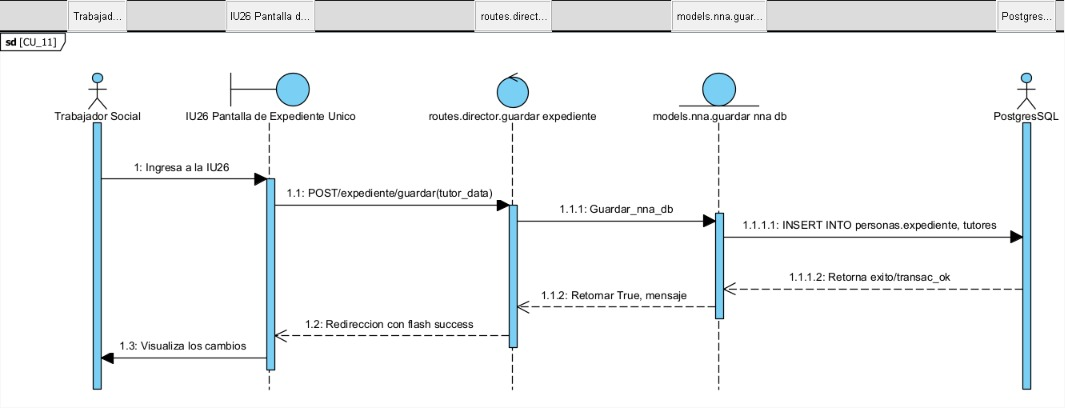
\includegraphics[width=0.85\textwidth]{CU/CU11.jpeg}
\caption{Diagrama de secuencia para el Caso de Uso de Registrar Cuidador / Tutor.}
\label{fig:secuenciaCU11}
\end{figure}

\subsection{Descripción de las Interacciones}
\begin{enumerate}
    \item El Trabajador Social llena los campos del formulario del tutor en la pestaña del expediente único y presiona \textit{Guardar}. Esto envía una petición POST al controlador del expediente.
    \item El controlador (\texttt{routes.director.guardar\_expediente}) recibe los datos del tutor (nombre, CURP, ocupación, parentesco, etc.) y llama al modelo de negocio (\texttt{models.nna.guardar\_nna\_db}).
    \item El modelo abre una transacción y realiza la inserción de la persona del tutor en la tabla \texttt{personas\_expediente} para obtener su identificador, y posteriormente inserta los datos específicos del tutor en la tabla \texttt{tutores}.
    \item La base de datos guarda los datos y confirma el estado de la transacción.
    \item El modelo retorna un valor booleano de éxito al controlador.
    \item El controlador recarga la vista del expediente con un mensaje de éxito.
\end{enumerate}

%---------------------------------------------------------
\section{Diseño dinámico del CU-12: Registrar Familiar de NNA}
\label{sec:disenoDinamicoCU12}

Permite al Trabajador Social agregar familiares adicionales a la red familiar o de apoyo del menor en el expediente único.

\begin{figure}[htbp!]
\centering
\begin{tikzpicture}[
    node distance=1cm and 1.8cm,
    actor/.style={rectangle, draw, fill=blue!15, text width=2.5cm, text centered, rounded corners, minimum height=1cm, font=\sffamily\small},
    lifeline/.style={draw, dashed, thick},
    arrow/.style={thick,->,>=stealth,font=\sffamily\scriptsize},
    rarrow/.style={thick,->,>=stealth,dashed,font=\sffamily\scriptsize}
]
    % Lifelines / Objects
    \node (user) [actor] {Trabajador Social \\ (Browser)};
    \node (router) [actor, right=of user] {Controlador \\ (routes.director)};
    \node (model) [actor, right=of router] {Modelo \\ (models.nna)};
    \node (db) [actor, right=of model] {Base de Datos \\ (PostgreSQL)};
    % Lines
    \draw [lifeline] (user.south) -- ($(user.south) - (0,6cm)$);
    \draw [lifeline] (router.south) -- ($(router.south) - (0,6cm)$);
    \draw [lifeline] (model.south) -- ($(model.south) - (0,6cm)$);
    \draw [lifeline] (db.south) -- ($(db.south) - (0,6cm)$);
    % Steps
    \draw [arrow] ($(user.south) - (0,0.5cm)$) -- node[above] {1. POST /expediente/guardar (familiar\_data)} ($(router.south) - (0,0.5cm)$);
    \draw [arrow] ($(router.south) - (0,1.5cm)$) -- node[above] {2. guardar\_nna\_db(datos)} ($(model.south) - (0,1.5cm)$);
    \draw [arrow] ($(model.south) - (0,2.5cm)$) -- node[above] {3. INSERT INTO personas\_expediente, familiares} ($(db.south) - (0,2.5cm)$);
    \draw [rarrow] ($(db.south) - (0,3.5cm)$) -- node[above] {4. Retorna éxito / transac\_ok} ($(model.south) - (0,3.5cm)$);
    \draw [rarrow] ($(model.south) - (0,4.5cm)$) -- node[above] {5. Retorna True, mensaje} ($(router.south) - (0,4.5cm)$);
    \draw [rarrow] ($(router.south) - (0,5.5cm)$) -- node[above] {6. Redirección con flash success} ($(user.south) - (0,5.5cm)$);
\end{tikzpicture}
\caption{Diagrama de secuencia para el Caso de Uso de Registrar Familiar de NNA.}
\label{fig:secuenciaCU12}
\end{figure}

\subsection{Descripción de las Interacciones}
\begin{enumerate}
    \item El Trabajador Social presiona el botón para añadir familiar en el entorno familiar del menor, captura la información en el formulario y lo envía por POST.
    \item El controlador intercepta los datos y los pasa al modelo \texttt{guardar\_nna\_db} para su registro.
    \item El modelo realiza la inserción en \texttt{personas\_expediente} para los datos generales del familiar, y posteriormente asocia el registro en la tabla \texttt{familiares} de la base de datos PostgreSQL.
    \item La base de datos confirma el guardado seguro.
    \item El modelo prorroga el éxito del registro al controlador de la ruta.
    \item El controlador refresca la vista del expediente confirmando el registro del familiar.
\end{enumerate}

%---------------------------------------------------------
\section{Diseño dinámico del CU-13: Consultar Alertas y Notificaciones}
\label{sec:disenoDinamicoCU13}

Permite a cualquier usuario conectado en el panel visualizar la bandeja de alertas y notificaciones del sistema asociadas a plazos.

\begin{figure}[htbp!]
\centering
\begin{tikzpicture}[
    node distance=1cm and 1.8cm,
    actor/.style={rectangle, draw, fill=blue!15, text width=2.5cm, text centered, rounded corners, minimum height=1cm, font=\sffamily\small},
    lifeline/.style={draw, dashed, thick},
    arrow/.style={thick,->,>=stealth,font=\sffamily\scriptsize},
    rarrow/.style={thick,->,>=stealth,dashed,font=\sffamily\scriptsize}
]
    % Lifelines / Objects
    \node (user) [actor] {Usuario \\ (Browser)};
    \node (router) [actor, right=of user] {Controlador \\ (routes.director)};
    \node (model) [actor, right=of router] {Modelo \\ (models.nna)};
    \node (db) [actor, right=of model] {Base de Datos \\ (PostgreSQL)};
    % Lines
    \draw [lifeline] (user.south) -- ($(user.south) - (0,6cm)$);
    \draw [lifeline] (router.south) -- ($(router.south) - (0,6cm)$);
    \draw [lifeline] (model.south) -- ($(model.south) - (0,6cm)$);
    \draw [lifeline] (db.south) -- ($(db.south) - (0,6cm)$);
    % Steps
    \draw [arrow] ($(user.south) - (0,0.5cm)$) -- node[above] {1. GET /director/dashboard} ($(router.south) - (0,0.5cm)$);
    \draw [arrow] ($(router.south) - (0,1.5cm)$) -- node[above] {2. Obtener alertas por CURP y rol} ($(model.south) - (0,1.5cm)$);
    \draw [arrow] ($(model.south) - (0,2.5cm)$) -- node[above] {3. SELECT ... FROM expediente WHERE ...} ($(db.south) - (0,2.5cm)$);
    \draw [rarrow] ($(db.south) - (0,3.5cm)$) -- node[above] {4. Retorna filas de vigencias y plazos} ($(model.south) - (0,3.5cm)$);
    \draw [rarrow] ($(model.south) - (0,4.5cm)$) -- node[above] {5. Retorna bandeja formateada} ($(router.south) - (0,4.5cm)$);
    \draw [rarrow] ($(router.south) - (0,5.5cm)$) -- node[above] {6. Renderiza dashboard con notificaciones} ($(user.south) - (0,5.5cm)$);
\end{tikzpicture}
\caption{Diagrama de secuencia para el Caso de Uso de Consultar Alertas y Notificaciones.}
\label{fig:secuenciaCU13}
\end{figure}

\subsection{Descripción de las Interacciones}
\begin{enumerate}
    \item El usuario ingresa a su Dashboard principal o hace clic en el apartado de alertas en el panel superior.
    \item El controlador recupera los datos de la sesión del usuario (CURP y Rol) y hace una petición al modelo para consultar las alertas y notificaciones del sistema correspondientes.
    \item El modelo calcula las vigencias y plazos ejecutando una consulta SQL sobre la tabla \texttt{expediente} y tablas de seguimiento de medidas en la base de datos PostgreSQL.
    \item El gestor PostgreSQL procesa la consulta y retorna las filas con los plazos calculados.
    \item El modelo procesa y retorna la bandeja de alertas estructurada (clasificada con semáforo por nivel de urgencia).
    \item El controlador recibe la información y renderiza el panel principal desplegando la bandeja de notificaciones al usuario.
\end{enumerate}



%---------------------------------------------------------
\cleardoublepage
\section{Diseño dinámico del CU-14: Elaborar y aprobar el Plan de Restitución de Derechos (PRD)}
\label{sec:disenoDinamicoCU14}

Permite al Coordinador de Caso consolidar el cuadro guía del PRD a partir de las valoraciones registradas por los especialistas, enviarlo a pre-autorización, y permite al Director autorizarlo y firmarlo digitalmente.

\begin{figure}[htbp!]
\centering
\begin{tikzpicture}[
    node distance=1cm and 1.8cm,
    actor/.style={rectangle, draw, fill=blue!15, text width=2.5cm, text centered, rounded corners, minimum height=1cm, font=\sffamily\small},
    lifeline/.style={draw, dashed, thick},
    arrow/.style={thick,->,>=stealth,font=\sffamily\scriptsize},
    rarrow/.style={thick,->,>=stealth,dashed,font=\sffamily\scriptsize}
]
    % Lifelines / Objects
    \node (user) [actor] {Coordinador \\ (Browser)};
    \node (router) [actor, right=of user] {Controlador \\ (routes.coordinador)};
    \node (model) [actor, right=of router] {Modelo \\ (models.nna)};
    \node (db) [actor, right=of model] {Base de Datos \\ (PostgreSQL)};
    % Lines
    \draw [lifeline] (user.south) -- ($(user.south) - (0,6cm)$);
    \draw [lifeline] (router.south) -- ($(router.south) - (0,6cm)$);
    \draw [lifeline] (model.south) -- ($(model.south) - (0,6cm)$);
    \draw [lifeline] (db.south) -- ($(db.south) - (0,6cm)$);
    % Steps
    \draw [arrow] ($(user.south) - (0,0.5cm)$) -- node[above] {1. POST /prd/guardar} ($(router.south) - (0,0.5cm)$);
    \draw [arrow] ($(router.south) - (0,1.5cm)$) -- node[above] {2. save\_prd(datos)} ($(model.south) - (0,1.5cm)$);
    \draw [arrow] ($(model.south) - (0,2.5cm)$) -- node[above] {3. INSERT INTO plan\_restitucion} ($(db.south) - (0,2.5cm)$);
    \draw [rarrow] ($(db.south) - (0,3.5cm)$) -- node[above] {4. Retorna id\_plan} ($(model.south) - (0,3.5cm)$);
    \draw [rarrow] ($(model.south) - (0,4.5cm)$) -- node[above] {5. Retorna True} ($(router.south) - (0,4.5cm)$);
    \draw [rarrow] ($(router.south) - (0,5.5cm)$) -- node[above] {6. Redirecciona con exito} ($(user.south) - (0,5.5cm)$);
\end{tikzpicture}
\caption{Diagrama de secuencia para el Caso de Uso de Elaborar y aprobar el Plan de Restitución de Derechos (PRD).}
\label{fig:secuenciaCU14}
\end{figure}

\subsection{Descripción de las Interacciones}
\begin{enumerate}
    \item El Coordinador ingresa a la sección del PRD en el panel del expediente.
    \item El controlador Flask (routes.coordinador) solicita al modelo (models.nna) las valoraciones de los especialistas para verificar precondiciones.
    \item El modelo ejecuta consultas SELECT en la base de datos PostgreSQL sobre las tablas de valoraciones.
    \item Si las valoraciones están completas, se habilita el formulario del PRD en la interfaz.
    \item El Coordinador registra el cuadro guía de medidas y presiona Guardar. El controlador persiste los datos en las tablas 'plan\_restitucion' y 'medidas\_prd'.
    \item El Director accede a la bandeja de firmas, revisa el PRD y lo firma digitalmente. El controlador actualiza el estatus del expediente a 'En Seguimiento' en la tabla 'expediente'.
\end{enumerate}

%---------------------------------------------------------
\cleardoublepage
\section{Diseño dinámico del CU-15: Registrar seguimiento de medidas de protección}
\label{sec:disenoDinamicoCU15}

Permite a los integrantes del equipo multidisciplinario actualizar el estatus de ejecución de cada medida de protección especial contenida en el PRD vigente, capturando bitácoras de avance y evidencias.

\begin{figure}[htbp!]
\centering
\begin{tikzpicture}[
    node distance=1cm and 1.8cm,
    actor/.style={rectangle, draw, fill=blue!15, text width=2.5cm, text centered, rounded corners, minimum height=1cm, font=\sffamily\small},
    lifeline/.style={draw, dashed, thick},
    arrow/.style={thick,->,>=stealth,font=\sffamily\scriptsize},
    rarrow/.style={thick,->,>=stealth,dashed,font=\sffamily\scriptsize}
]
    % Lifelines / Objects
    \node (user) [actor] {Especialista \\ (Browser)};
    \node (router) [actor, right=of user] {Controlador \\ (routes.coordinador)};
    \node (model) [actor, right=of router] {Modelo \\ (models.nna)};
    \node (db) [actor, right=of model] {Base de Datos \\ (PostgreSQL)};
    % Lines
    \draw [lifeline] (user.south) -- ($(user.south) - (0,6cm)$);
    \draw [lifeline] (router.south) -- ($(router.south) - (0,6cm)$);
    \draw [lifeline] (model.south) -- ($(model.south) - (0,6cm)$);
    \draw [lifeline] (db.south) -- ($(db.south) - (0,6cm)$);
    % Steps
    \draw [arrow] ($(user.south) - (0,0.5cm)$) -- node[above] {1. POST /medida/seguimiento} ($(router.south) - (0,0.5cm)$);
    \draw [arrow] ($(router.south) - (0,1.5cm)$) -- node[above] {2. update\_medida(datos)} ($(model.south) - (0,1.5cm)$);
    \draw [arrow] ($(model.south) - (0,2.5cm)$) -- node[above] {3. INSERT INTO bitacora\_medidas} ($(db.south) - (0,2.5cm)$);
    \draw [rarrow] ($(db.south) - (0,3.5cm)$) -- node[above] {4. Retorna ok} ($(model.south) - (0,3.5cm)$);
    \draw [rarrow] ($(model.south) - (0,4.5cm)$) -- node[above] {5. Retorna True} ($(router.south) - (0,4.5cm)$);
    \draw [rarrow] ($(router.south) - (0,5.5cm)$) -- node[above] {6. Redirección con exito} ($(user.south) - (0,5.5cm)$);
\end{tikzpicture}
\caption{Diagrama de secuencia para el Caso de Uso de Registrar seguimiento de medidas de protección.}
\label{fig:secuenciaCU15}
\end{figure}

\subsection{Descripción de las Interacciones}
\begin{enumerate}
    \item El especialista ingresa a la sección de seguimiento de medidas del expediente.
    \item El controlador Flask (routes.coordinador) recupera la lista de medidas vigentes llamando al modelo (models.nna).
    \item El especialista selecciona una medida, captura las observaciones, adjunta evidencia y presiona Guardar.
    \item El controlador guarda la evidencia física en el servidor y registra la ruta en la tabla 'documentos\_nna'.
    \item El modelo inserta la bitácora de seguimiento en la tabla 'bitacora\_medidas' de PostgreSQL.
    \item El sistema verifica si todas las medidas del PRD están en estatus 'Cumplida' para habilitar la opción de cierre del expediente.
\end{enumerate}

%---------------------------------------------------------
\cleardoublepage
\section{Diseño dinámico del CU-16: Capturar ficha de verificación del cumplimiento de derechos}
\label{sec:disenoDinamicoCU16}

Permite a los integrantes del equipo multidisciplinario completar la ficha de verificación de cumplimiento de derechos de la LGDNNA, identificando de manera estructurada los derechos vulnerados.

\begin{figure}[htbp!]
\centering
\begin{tikzpicture}[
    node distance=1cm and 1.8cm,
    actor/.style={rectangle, draw, fill=blue!15, text width=2.5cm, text centered, rounded corners, minimum height=1cm, font=\sffamily\small},
    lifeline/.style={draw, dashed, thick},
    arrow/.style={thick,->,>=stealth,font=\sffamily\scriptsize},
    rarrow/.style={thick,->,>=stealth,dashed,font=\sffamily\scriptsize}
]
    % Lifelines / Objects
    \node (user) [actor] {Especialista \\ (Browser)};
    \node (router) [actor, right=of user] {Controlador \\ (routes.coordinador)};
    \node (model) [actor, right=of router] {Modelo \\ (models.nna)};
    \node (db) [actor, right=of model] {Base de Datos \\ (PostgreSQL)};
    % Lines
    \draw [lifeline] (user.south) -- ($(user.south) - (0,6cm)$);
    \draw [lifeline] (router.south) -- ($(router.south) - (0,6cm)$);
    \draw [lifeline] (model.south) -- ($(model.south) - (0,6cm)$);
    \draw [lifeline] (db.south) -- ($(db.south) - (0,6cm)$);
    % Steps
    \draw [arrow] ($(user.south) - (0,0.5cm)$) -- node[above] {1. POST /expediente/verificacion} ($(router.south) - (0,0.5cm)$);
    \draw [arrow] ($(router.south) - (0,1.5cm)$) -- node[above] {2. save\_verificacion(datos)} ($(model.south) - (0,1.5cm)$);
    \draw [arrow] ($(model.south) - (0,2.5cm)$) -- node[above] {3. INSERT INTO ficha\_verificacion} ($(db.south) - (0,2.5cm)$);
    \draw [rarrow] ($(db.south) - (0,3.5cm)$) -- node[above] {4. Retorna ok} ($(model.south) - (0,3.5cm)$);
    \draw [rarrow] ($(model.south) - (0,4.5cm)$) -- node[above] {5. Retorna True} ($(router.south) - (0,4.5cm)$);
    \draw [rarrow] ($(router.south) - (0,5.5cm)$) -- node[above] {6. Muestra exito} ($(user.south) - (0,5.5cm)$);
\end{tikzpicture}
\caption{Diagrama de secuencia para el Caso de Uso de Capturar ficha de verificación del cumplimiento de derechos.}
\label{fig:secuenciaCU16}
\end{figure}

\subsection{Descripción de las Interacciones}
\begin{enumerate}
    \item El especialista accede al expediente y selecciona la pestaña Ficha de Verificación.
    \item El controlador valida que el especialista pertenezca al equipo multidisciplinario asignado al caso.
    \item El especialista responde a los elementos de evaluación (Si/No/No aplica) de cada categoría y guarda.
    \item El controlador (routes.coordinador) envía los datos al modelo para su almacenamiento.
    \item El modelo persiste los registros en la tabla 'ficha\_verificacion' y asocia los derechos vulnerados (marcados como No) en la lista de sugerencias para el PRD.
\end{enumerate}

%---------------------------------------------------------
\cleardoublepage
\section{Diseño dinámico del CU-17: Registrar detección inicial de caso}
\label{sec:disenoDinamicoCU17}

Permite al Coordinador o especialista capturar el formato de registro de detección de un posible caso de vulneración de derechos, previo a la apertura formal del expediente.

\begin{figure}[htbp!]
\centering
\begin{tikzpicture}[
    node distance=1cm and 1.8cm,
    actor/.style={rectangle, draw, fill=blue!15, text width=2.5cm, text centered, rounded corners, minimum height=1cm, font=\sffamily\small},
    lifeline/.style={draw, dashed, thick},
    arrow/.style={thick,->,>=stealth,font=\sffamily\scriptsize},
    rarrow/.style={thick,->,>=stealth,dashed,font=\sffamily\scriptsize}
]
    % Lifelines / Objects
    \node (user) [actor] {Usuario \\ (Browser)};
    \node (router) [actor, right=of user] {Controlador \\ (routes.coordinador)};
    \node (model) [actor, right=of router] {Modelo \\ (models.nna)};
    \node (db) [actor, right=of model] {Base de Datos \\ (PostgreSQL)};
    % Lines
    \draw [lifeline] (user.south) -- ($(user.south) - (0,6cm)$);
    \draw [lifeline] (router.south) -- ($(router.south) - (0,6cm)$);
    \draw [lifeline] (model.south) -- ($(model.south) - (0,6cm)$);
    \draw [lifeline] (db.south) -- ($(db.south) - (0,6cm)$);
    % Steps
    \draw [arrow] ($(user.south) - (0,0.5cm)$) -- node[above] {1. POST /deteccion/registrar} ($(router.south) - (0,0.5cm)$);
    \draw [arrow] ($(router.south) - (0,1.5cm)$) -- node[above] {2. create\_detection(datos)} ($(model.south) - (0,1.5cm)$);
    \draw [arrow] ($(model.south) - (0,2.5cm)$) -- node[above] {3. INSERT INTO hecho\_victimal} ($(db.south) - (0,2.5cm)$);
    \draw [rarrow] ($(db.south) - (0,3.5cm)$) -- node[above] {4. Retorna num\_reporte} ($(model.south) - (0,3.5cm)$);
    \draw [rarrow] ($(model.south) - (0,4.5cm)$) -- node[above] {5. Retorna num\_reporte} ($(router.south) - (0,4.5cm)$);
    \draw [rarrow] ($(router.south) - (0,5.5cm)$) -- node[above] {6. Redirecciona con exito} ($(user.south) - (0,5.5cm)$);
\end{tikzpicture}
\caption{Diagrama de secuencia para el Caso de Uso de Registrar detección inicial de caso.}
\label{fig:secuenciaCU17}
\end{figure}

\subsection{Descripción de las Interacciones}
\begin{enumerate}
    \item El usuario selecciona la opción para registrar una detección de caso en el panel.
    \item El controlador Flask despliega el formato con los campos de descripción y datos de aviso.
    \item El usuario captura los datos y presiona Guardar.
    \item El controlador (routes.coordinador) llama al modelo de registro de casos.
    \item El modelo genera un número de reporte consecutivo automático y lo inserta en la tabla 'deteccion\_caso' de PostgreSQL.
    \item El sistema muestra el folio generado en pantalla y ofrece la opción de crear el expediente del menor.
\end{enumerate}

%---------------------------------------------------------
\cleardoublepage
\section{Diseño dinámico del CU-18: Cerrar expediente del NNA}
\label{sec:disenoDinamicoCU18}

Permite al Coordinador solicitar el cierre del expediente una vez que todas las medidas han sido cumplidas, y permite al Director validar y autorizar el cierre definitivo.

\begin{figure}[htbp!]
\centering
\begin{tikzpicture}[
    node distance=1cm and 1.8cm,
    actor/.style={rectangle, draw, fill=blue!15, text width=2.5cm, text centered, rounded corners, minimum height=1cm, font=\sffamily\small},
    lifeline/.style={draw, dashed, thick},
    arrow/.style={thick,->,>=stealth,font=\sffamily\scriptsize},
    rarrow/.style={thick,->,>=stealth,dashed,font=\sffamily\scriptsize}
]
    % Lifelines / Objects
    \node (user) [actor] {Usuario \\ (Browser)};
    \node (router) [actor, right=of user] {Controlador \\ (routes.director)};
    \node (model) [actor, right=of router] {Modelo \\ (models.nna)};
    \node (db) [actor, right=of model] {Base de Datos \\ (PostgreSQL)};
    % Lines
    \draw [lifeline] (user.south) -- ($(user.south) - (0,6cm)$);
    \draw [lifeline] (router.south) -- ($(router.south) - (0,6cm)$);
    \draw [lifeline] (model.south) -- ($(model.south) - (0,6cm)$);
    \draw [lifeline] (db.south) -- ($(db.south) - (0,6cm)$);
    % Steps
    \draw [arrow] ($(user.south) - (0,0.5cm)$) -- node[above] {1. POST /expediente/cerrar} ($(router.south) - (0,0.5cm)$);
    \draw [arrow] ($(router.south) - (0,1.5cm)$) -- node[above] {2. close\_expediente(id)} ($(model.south) - (0,1.5cm)$);
    \draw [arrow] ($(model.south) - (0,2.5cm)$) -- node[above] {3. UPDATE expediente SET estado = \%s} ($(db.south) - (0,2.5cm)$);
    \draw [rarrow] ($(db.south) - (0,3.5cm)$) -- node[above] {4. Retorna ok} ($(model.south) - (0,3.5cm)$);
    \draw [rarrow] ($(model.south) - (0,4.5cm)$) -- node[above] {5. Retorna True} ($(router.south) - (0,4.5cm)$);
    \draw [rarrow] ($(router.south) - (0,5.5cm)$) -- node[above] {6. Redirecciona con exito} ($(user.south) - (0,5.5cm)$);
\end{tikzpicture}
\caption{Diagrama de secuencia para el Caso de Uso de Cerrar expediente del NNA.}
\label{fig:secuenciaCU18}
\end{figure}

\subsection{Descripción de las Interacciones}
\begin{enumerate}
    \item El Coordinador presiona la opción para solicitar el cierre de un expediente.
    \item El controlador verifica que todas las medidas del PRD del expediente estén registradas como cumplidas.
    \item El Coordinador ingresa la justificación del cierre y presiona Enviar.
    \item El sistema actualiza el estatus del expediente a 'Cierre Solicitado' en la tabla 'expediente'.
    \item El Director revisa la solicitud en su bandeja de control y autoriza el cierre. El controlador actualiza el estatus a 'Cerrado' e inhabilita las ediciones del expediente (modo de solo lectura).
\end{enumerate}

%---------------------------------------------------------
\cleardoublepage
\section{Diseño dinámico del CU-19: Recuperar contraseña}
\label{sec:disenoDinamicoCU19}

Permite a cualquier usuario registrado solicitar el restablecimiento de su contraseña mediante el envío de un enlace de recuperación a su correo institucional registrado.

\begin{figure}[htbp!]
\centering
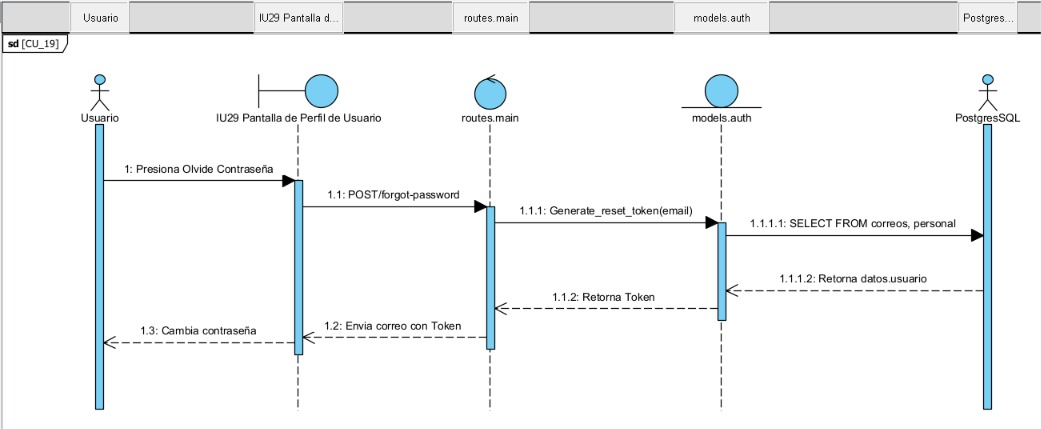
\includegraphics[width=0.85\textwidth]{CU/CU19.jpeg}
\caption{Diagrama de secuencia para el Caso de Uso de Recuperar contraseña.}
\label{fig:secuenciaCU19}
\end{figure}

\subsection{Descripción de las Interacciones}
\begin{enumerate}
    \item El usuario hace clic en el enlace 'Olvidaste tu contraseña' en la pantalla de login.
    \item Ingresa su correo institucional y envía el formulario.
    \item El controlador (routes.main) llama a la función del modelo de autenticación.
    \item El modelo busca el correo en la tabla 'correos' de la base de datos para validar su existencia.
    \item El sistema genera un token de un solo uso, lo registra en la base de datos con una fecha de expiración y envía un correo con el enlace de restablecimiento al usuario.
\end{enumerate}

%---------------------------------------------------------
\cleardoublepage
\section{Diseño dinámico del CU-20: Cambiar contraseña}
\label{sec:disenoDinamicoCU20}

Permite a cualquier usuario autenticado actualizar su contraseña de acceso al sistema desde la pantalla de su perfil de cuenta.

\begin{figure}[htbp!]
\centering
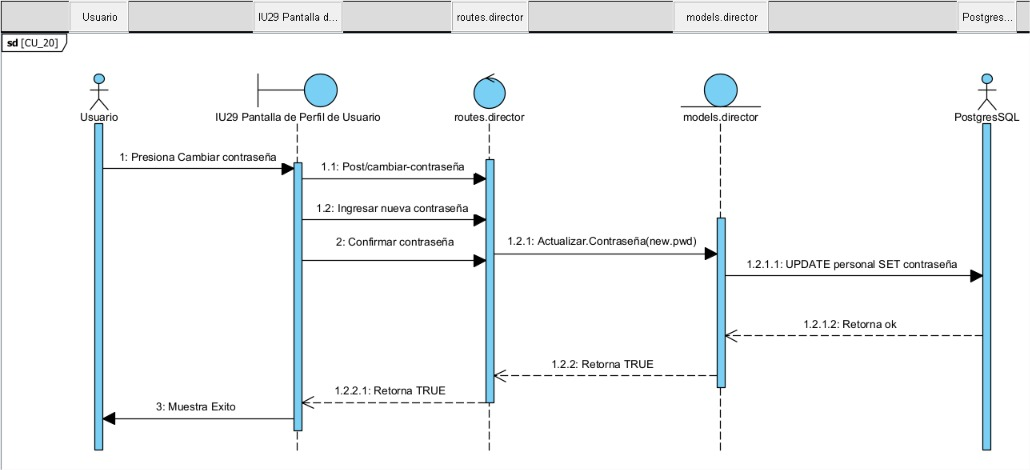
\includegraphics[width=0.85\textwidth]{CU/CU20.jpeg}
\caption{Diagrama de secuencia para el Caso de Uso de Cambiar contraseña.}
\label{fig:secuenciaCU20}
\end{figure}

\subsection{Descripción de las Interacciones}
\begin{enumerate}
    \item El usuario accede a su perfil y selecciona la opción de cambiar contraseña.
    \item Ingresa la contraseña actual, la nueva contraseña y la confirmación.
    \item El controlador verifica que la contraseña actual ingresada coincida con la registrada en la tabla 'personal'.
    \item El sistema valida que la nueva contraseña cumpla con los requisitos mínimos de seguridad y que coincida con la confirmación.
    \item El modelo actualiza el hash de la contraseña en la tabla 'personal' de PostgreSQL y despliega un mensaje de éxito.
\end{enumerate}

%---------------------------------------------------------
\cleardoublepage
\section{Diseño dinámico del CU-21: Buscar y filtrar expedientes}
\label{sec:disenoDinamicoCU21}

Permite a cualquier usuario autenticado localizar expedientes de NNA mediante búsqueda por nombre, CURP o folio, y filtrarlos por estado o rango de fechas.

\begin{figure}[htbp!]
\centering
\begin{tikzpicture}[
    node distance=1cm and 1.8cm,
    actor/.style={rectangle, draw, fill=blue!15, text width=2.5cm, text centered, rounded corners, minimum height=1cm, font=\sffamily\small},
    lifeline/.style={draw, dashed, thick},
    arrow/.style={thick,->,>=stealth,font=\sffamily\scriptsize},
    rarrow/.style={thick,->,>=stealth,dashed,font=\sffamily\scriptsize}
]
    % Lifelines / Objects
    \node (user) [actor] {Usuario \\ (Browser)};
    \node (router) [actor, right=of user] {Controlador \\ (routes.coordinador)};
    \node (model) [actor, right=of router] {Modelo \\ (models.nna)};
    \node (db) [actor, right=of model] {Base de Datos \\ (PostgreSQL)};
    % Lines
    \draw [lifeline] (user.south) -- ($(user.south) - (0,6cm)$);
    \draw [lifeline] (router.south) -- ($(router.south) - (0,6cm)$);
    \draw [lifeline] (model.south) -- ($(model.south) - (0,6cm)$);
    \draw [lifeline] (db.south) -- ($(db.south) - (0,6cm)$);
    % Steps
    \draw [arrow] ($(user.south) - (0,0.5cm)$) -- node[above] {1. GET /expedientes (query, filtros)} ($(router.south) - (0,0.5cm)$);
    \draw [arrow] ($(router.south) - (0,1.5cm)$) -- node[above] {2. get\_expedientes\_filtered(filtros)} ($(model.south) - (0,1.5cm)$);
    \draw [arrow] ($(model.south) - (0,2.5cm)$) -- node[above] {3. SELECT FROM personas\_expediente} ($(db.south) - (0,2.5cm)$);
    \draw [rarrow] ($(db.south) - (0,3.5cm)$) -- node[above] {4. Retorna filas coincidentes} ($(model.south) - (0,3.5cm)$);
    \draw [rarrow] ($(model.south) - (0,4.5cm)$) -- node[above] {5. Retorna lista de dicts} ($(router.south) - (0,4.5cm)$);
    \draw [rarrow] ($(router.south) - (0,5.5cm)$) -- node[above] {6. Renderiza lista en panel} ($(user.south) - (0,5.5cm)$);
\end{tikzpicture}
\caption{Diagrama de secuencia para el Caso de Uso de Buscar y filtrar expedientes.}
\label{fig:secuenciaCU21}
\end{figure}

\subsection{Descripción de las Interacciones}
\begin{enumerate}
    \item El usuario ingresa al panel de expedientes.
    \item El controlador recupera el rol y equipo del usuario para restringir la consulta inicial.
    \item El usuario captura un texto de búsqueda (nombre, CURP o folio) y/o selecciona filtros.
    \item El controlador realiza una consulta dinámica llamando al modelo de búsqueda.
    \item El modelo ejecuta un query SELECT con filtros ILIKE y operadores lógicos sobre la tabla 'personas\_expediente' y 'expediente' en PostgreSQL.
    \item El controlador recibe la lista filtrada de expedientes y la renderiza paginada en pantalla.
\end{enumerate}

%---------------------------------------------------------
\cleardoublepage
\section{Diseño dinámico del CU-22: Registrar datos médicos del NNA}
\label{sec:disenoDinamicoCU22}

Permite al Médico capturar el historial clínico inicial del NNA en el expediente: seguro médico, padecimientos, cartilla, discapacidades y alimentación.

\begin{figure}[htbp!]
\centering
\begin{tikzpicture}[
    node distance=1cm and 1.8cm,
    actor/.style={rectangle, draw, fill=blue!15, text width=2.5cm, text centered, rounded corners, minimum height=1cm, font=\sffamily\small},
    lifeline/.style={draw, dashed, thick},
    arrow/.style={thick,->,>=stealth,font=\sffamily\scriptsize},
    rarrow/.style={thick,->,>=stealth,dashed,font=\sffamily\scriptsize}
]
    % Lifelines / Objects
    \node (user) [actor] {Médico \\ (Browser)};
    \node (router) [actor, right=of user] {Controlador \\ (routes.coordinador)};
    \node (model) [actor, right=of router] {Modelo \\ (models.nna)};
    \node (db) [actor, right=of model] {Base de Datos \\ (PostgreSQL)};
    % Lines
    \draw [lifeline] (user.south) -- ($(user.south) - (0,6cm)$);
    \draw [lifeline] (router.south) -- ($(router.south) - (0,6cm)$);
    \draw [lifeline] (model.south) -- ($(model.south) - (0,6cm)$);
    \draw [lifeline] (db.south) -- ($(db.south) - (0,6cm)$);
    % Steps
    \draw [arrow] ($(user.south) - (0,0.5cm)$) -- node[above] {1. POST /medico/guardar} ($(router.south) - (0,0.5cm)$);
    \draw [arrow] ($(router.south) - (0,1.5cm)$) -- node[above] {2. save\_datos\_medicos(datos)} ($(model.south) - (0,1.5cm)$);
    \draw [arrow] ($(model.south) - (0,2.5cm)$) -- node[above] {3. INSERT INTO nna\_padecimientos} ($(db.south) - (0,2.5cm)$);
    \draw [rarrow] ($(db.south) - (0,3.5cm)$) -- node[above] {4. Retorna ok} ($(model.south) - (0,3.5cm)$);
    \draw [rarrow] ($(model.south) - (0,4.5cm)$) -- node[above] {5. Retorna True} ($(router.south) - (0,4.5cm)$);
    \draw [rarrow] ($(router.south) - (0,5.5cm)$) -- node[above] {6. Redirecciona con exito} ($(user.south) - (0,5.5cm)$);
\end{tikzpicture}
\caption{Diagrama de secuencia para el Caso de Uso de Registrar datos médicos del NNA.}
\label{fig:secuenciaCU22}
\end{figure}

\subsection{Descripción de las Interacciones}
\begin{enumerate}
    \item El Médico accede a la pestaña Datos Médicos del expediente unificado.
    \item El controlador Flask valida la asignación del Médico al equipo del expediente.
    \item El Médico captura la información y selecciona padecimientos del catálogo CIE-10 y discapacidades.
    \item Al guardar, el controlador invoca a la función del modelo (models.nna).
    \item El modelo realiza inserciones atómicas en las tablas 'nna\_seguro\_medico', 'nna\_padecimientos' y 'nna\_discapacidad' de la base de datos PostgreSQL.
    \item Se actualiza el indicador de valoración médica en el expediente a completada.
\end{enumerate}

%---------------------------------------------------------
\cleardoublepage
\section{Diseño dinámico del CU-23: Registrar valoración psicológica}
\label{sec:disenoDinamicoCU23}

Permite al Psicólogo registrar el diagnóstico del estado emocional del NNA, observaciones de comportamiento y notas terapéuticas.

\begin{figure}[htbp!]
\centering
\begin{tikzpicture}[
    node distance=1cm and 1.8cm,
    actor/.style={rectangle, draw, fill=blue!15, text width=2.5cm, text centered, rounded corners, minimum height=1cm, font=\sffamily\small},
    lifeline/.style={draw, dashed, thick},
    arrow/.style={thick,->,>=stealth,font=\sffamily\scriptsize},
    rarrow/.style={thick,->,>=stealth,dashed,font=\sffamily\scriptsize}
]
    % Lifelines / Objects
    \node (user) [actor] {Psicólogo \\ (Browser)};
    \node (router) [actor, right=of user] {Controlador \\ (routes.coordinador)};
    \node (model) [actor, right=of router] {Modelo \\ (models.nna)};
    \node (db) [actor, right=of model] {Base de Datos \\ (PostgreSQL)};
    % Lines
    \draw [lifeline] (user.south) -- ($(user.south) - (0,6cm)$);
    \draw [lifeline] (router.south) -- ($(router.south) - (0,6cm)$);
    \draw [lifeline] (model.south) -- ($(model.south) - (0,6cm)$);
    \draw [lifeline] (db.south) -- ($(db.south) - (0,6cm)$);
    % Steps
    \draw [arrow] ($(user.south) - (0,0.5cm)$) -- node[above] {1. POST /psicologo/guardar} ($(router.south) - (0,0.5cm)$);
    \draw [arrow] ($(router.south) - (0,1.5cm)$) -- node[above] {2. save\_valoracion\_psi(datos)} ($(model.south) - (0,1.5cm)$);
    \draw [arrow] ($(model.south) - (0,2.5cm)$) -- node[above] {3. INSERT INTO valoraciones (psi)} ($(db.south) - (0,2.5cm)$);
    \draw [rarrow] ($(db.south) - (0,3.5cm)$) -- node[above] {4. Retorna ok} ($(model.south) - (0,3.5cm)$);
    \draw [rarrow] ($(model.south) - (0,4.5cm)$) -- node[above] {5. Retorna True} ($(router.south) - (0,4.5cm)$);
    \draw [rarrow] ($(router.south) - (0,5.5cm)$) -- node[above] {6. Redirecciona con exito} ($(user.south) - (0,5.5cm)$);
\end{tikzpicture}
\caption{Diagrama de secuencia para el Caso de Uso de Registrar valoración psicológica.}
\label{fig:secuenciaCU23}
\end{figure}

\subsection{Descripción de las Interacciones}
\begin{enumerate}
    \item El Psicólogo selecciona la pestaña Valoración Psicológica en el expediente.
    \item El controlador valida los permisos del Psicólogo sobre el expediente.
    \item El Psicólogo registra la narrativa terapéutica, observaciones e indicadores de riesgo detectados.
    \item El controlador envía los datos al modelo para su almacenamiento.
    \item El modelo inserta los registros en la tabla 'valoraciones' y actualiza el estado de la valoración psicológica a completada.
\end{enumerate}

%---------------------------------------------------------
\cleardoublepage
\section{Diseño dinámico del CU-24: Registrar valoración jurídica}
\label{sec:disenoDinamicoCU24}

Permite al Abogado capturar la valoración jurídica del caso: delitos, instancias involucradas, estado de la fiscalía y verificación de actas.

\begin{figure}[htbp!]
\centering
\begin{tikzpicture}[
    node distance=1cm and 1.8cm,
    actor/.style={rectangle, draw, fill=blue!15, text width=2.5cm, text centered, rounded corners, minimum height=1cm, font=\sffamily\small},
    lifeline/.style={draw, dashed, thick},
    arrow/.style={thick,->,>=stealth,font=\sffamily\scriptsize},
    rarrow/.style={thick,->,>=stealth,dashed,font=\sffamily\scriptsize}
]
    % Lifelines / Objects
    \node (user) [actor] {Abogado \\ (Browser)};
    \node (router) [actor, right=of user] {Controlador \\ (routes.coordinador)};
    \node (model) [actor, right=of router] {Modelo \\ (models.nna)};
    \node (db) [actor, right=of model] {Base de Datos \\ (PostgreSQL)};
    % Lines
    \draw [lifeline] (user.south) -- ($(user.south) - (0,6cm)$);
    \draw [lifeline] (router.south) -- ($(router.south) - (0,6cm)$);
    \draw [lifeline] (model.south) -- ($(model.south) - (0,6cm)$);
    \draw [lifeline] (db.south) -- ($(db.south) - (0,6cm)$);
    % Steps
    \draw [arrow] ($(user.south) - (0,0.5cm)$) -- node[above] {1. POST /abogado/guardar} ($(router.south) - (0,0.5cm)$);
    \draw [arrow] ($(router.south) - (0,1.5cm)$) -- node[above] {2. save\_valoracion\_jur(datos)} ($(model.south) - (0,1.5cm)$);
    \draw [arrow] ($(model.south) - (0,2.5cm)$) -- node[above] {3. INSERT INTO valoraciones (jur)} ($(db.south) - (0,2.5cm)$);
    \draw [rarrow] ($(db.south) - (0,3.5cm)$) -- node[above] {4. Retorna ok} ($(model.south) - (0,3.5cm)$);
    \draw [rarrow] ($(model.south) - (0,4.5cm)$) -- node[above] {5. Retorna True} ($(router.south) - (0,4.5cm)$);
    \draw [rarrow] ($(router.south) - (0,5.5cm)$) -- node[above] {6. Redirecciona con exito} ($(user.south) - (0,5.5cm)$);
\end{tikzpicture}
\caption{Diagrama de secuencia para el Caso de Uso de Registrar valoración jurídica.}
\label{fig:secuenciaCU24}
\end{figure}

\subsection{Descripción de las Interacciones}
\begin{enumerate}
    \item El Abogado accede al panel de Valoración Jurídica del expediente.
    \item Captura los delitos, el número de expediente de fiscalía, las medidas penales propuestas y valida el acta de nacimiento.
    \item El controlador (routes.coordinador) invoca la función de persistencia del modelo.
    \item El modelo inserta la valoración en la tabla 'valoraciones' de PostgreSQL y actualiza la tabla 'acta\_nacimiento' marcándola como verificada.
    \item Se registra la completitud de la valoración jurídica en el expediente.
\end{enumerate}

%---------------------------------------------------------
\cleardoublepage
\section{Diseño dinámico del CU-25: Registrar valoración sociofamiliar}
\label{sec:disenoDinamicoCU25}

Permite al Trabajador Social capturar el diagnóstico del entorno social del NNA: estructura, vivienda, redes de apoyo y evaluación de cuidadores.

\begin{figure}[htbp!]
\centering
\begin{tikzpicture}[
    node distance=1cm and 1.8cm,
    actor/.style={rectangle, draw, fill=blue!15, text width=2.5cm, text centered, rounded corners, minimum height=1cm, font=\sffamily\small},
    lifeline/.style={draw, dashed, thick},
    arrow/.style={thick,->,>=stealth,font=\sffamily\scriptsize},
    rarrow/.style={thick,->,>=stealth,dashed,font=\sffamily\scriptsize}
]
    % Lifelines / Objects
    \node (user) [actor] {T. Social \\ (Browser)};
    \node (router) [actor, right=of user] {Controlador \\ (routes.coordinador)};
    \node (model) [actor, right=of router] {Modelo \\ (models.nna)};
    \node (db) [actor, right=of model] {Base de Datos \\ (PostgreSQL)};
    % Lines
    \draw [lifeline] (user.south) -- ($(user.south) - (0,6cm)$);
    \draw [lifeline] (router.south) -- ($(router.south) - (0,6cm)$);
    \draw [lifeline] (model.south) -- ($(model.south) - (0,6cm)$);
    \draw [lifeline] (db.south) -- ($(db.south) - (0,6cm)$);
    % Steps
    \draw [arrow] ($(user.south) - (0,0.5cm)$) -- node[above] {1. POST /tsocial/guardar} ($(router.south) - (0,0.5cm)$);
    \draw [arrow] ($(router.south) - (0,1.5cm)$) -- node[above] {2. save\_valoracion\_soc(datos)} ($(model.south) - (0,1.5cm)$);
    \draw [arrow] ($(model.south) - (0,2.5cm)$) -- node[above] {3. UPDATE tutores SET negacion = \%s} ($(db.south) - (0,2.5cm)$);
    \draw [rarrow] ($(db.south) - (0,3.5cm)$) -- node[above] {4. Retorna ok} ($(model.south) - (0,3.5cm)$);
    \draw [rarrow] ($(model.south) - (0,4.5cm)$) -- node[above] {5. Retorna True} ($(router.south) - (0,4.5cm)$);
    \draw [rarrow] ($(router.south) - (0,5.5cm)$) -- node[above] {6. Redirecciona con exito} ($(user.south) - (0,5.5cm)$);
\end{tikzpicture}
\caption{Diagrama de secuencia para el Caso de Uso de Registrar valoración sociofamiliar.}
\label{fig:secuenciaCU25}
\end{figure}

\subsection{Descripción de las Interacciones}
\begin{enumerate}
    \item El Trabajador Social selecciona la pestaña Entorno Familiar en el expediente.
    \item Registra el sistema de residencia, dinámica, redes de apoyo y evalúa la negación y afectación del cuidador.
    \item Al guardar, el controlador envía los datos al modelo.
    \item El modelo actualiza los datos en la tabla 'tutores' y registra la valoración sociofamiliar en la tabla 'valoraciones'.
    \item Se actualiza el indicador sociofamiliar en el expediente a completado.
\end{enumerate}

%---------------------------------------------------------
\cleardoublepage
\section{Diseño dinámico del CU-26: Registrar observaciones de la entrevista con el NNA}
\label{sec:disenoDinamicoCU26}

Permite al Trabajador Social o Psicólogo registrar la actitud, tono de voz, expresión corporal y checklist de vida cotidiana de la entrevista con el menor.

\begin{figure}[htbp!]
\centering
\begin{tikzpicture}[
    node distance=1cm and 1.8cm,
    actor/.style={rectangle, draw, fill=blue!15, text width=2.5cm, text centered, rounded corners, minimum height=1cm, font=\sffamily\small},
    lifeline/.style={draw, dashed, thick},
    arrow/.style={thick,->,>=stealth,font=\sffamily\scriptsize},
    rarrow/.style={thick,->,>=stealth,dashed,font=\sffamily\scriptsize}
]
    % Lifelines / Objects
    \node (user) [actor] {Usuario \\ (Browser)};
    \node (router) [actor, right=of user] {Controlador \\ (routes.coordinador)};
    \node (model) [actor, right=of router] {Modelo \\ (models.nna)};
    \node (db) [actor, right=of model] {Base de Datos \\ (PostgreSQL)};
    % Lines
    \draw [lifeline] (user.south) -- ($(user.south) - (0,6cm)$);
    \draw [lifeline] (router.south) -- ($(router.south) - (0,6cm)$);
    \draw [lifeline] (model.south) -- ($(model.south) - (0,6cm)$);
    \draw [lifeline] (db.south) -- ($(db.south) - (0,6cm)$);
    % Steps
    \draw [arrow] ($(user.south) - (0,0.5cm)$) -- node[above] {1. POST /entrevista/guardar} ($(router.south) - (0,0.5cm)$);
    \draw [arrow] ($(router.south) - (0,1.5cm)$) -- node[above] {2. save\_entrevista\_obs(datos)} ($(model.south) - (0,1.5cm)$);
    \draw [arrow] ($(model.south) - (0,2.5cm)$) -- node[above] {3. INSERT INTO entrevista\_nna} ($(db.south) - (0,2.5cm)$);
    \draw [rarrow] ($(db.south) - (0,3.5cm)$) -- node[above] {4. Retorna ok} ($(model.south) - (0,3.5cm)$);
    \draw [rarrow] ($(model.south) - (0,4.5cm)$) -- node[above] {5. Retorna True} ($(router.south) - (0,4.5cm)$);
    \draw [rarrow] ($(router.south) - (0,5.5cm)$) -- node[above] {6. Muestra exito en pantalla} ($(user.south) - (0,5.5cm)$);
\end{tikzpicture}
\caption{Diagrama de secuencia para el Caso de Uso de Registrar observaciones de la entrevista con el NNA.}
\label{fig:secuenciaCU26}
\end{figure}

\subsection{Descripción de las Interacciones}
\begin{enumerate}
    \item El especialista ingresa a la pestaña Entrevista con NNA.
    \item Captura la narrativa de la actitud, tono de voz, expresión y responde al checklist de vida del menor.
    \item El controlador recibe los datos y los pasa al modelo de negocio.
    \item El modelo guarda la información en la tabla 'entrevista\_nna' de PostgreSQL.
    \item El sistema confirma el guardado y refresca la vista del expediente.
\end{enumerate}

%---------------------------------------------------------
\cleardoublepage
\section{Diseño dinámico del CU-27: Registrar familiograma del NNA}
\label{sec:disenoDinamicoCU27}

Permite al Trabajador Social construir y guardar la descripción textual y la imagen digitalizada del familiograma elaborado durante la entrevista.

\begin{figure}[htbp!]
\centering
\begin{tikzpicture}[
    node distance=1cm and 1.8cm,
    actor/.style={rectangle, draw, fill=blue!15, text width=2.5cm, text centered, rounded corners, minimum height=1cm, font=\sffamily\small},
    lifeline/.style={draw, dashed, thick},
    arrow/.style={thick,->,>=stealth,font=\sffamily\scriptsize},
    rarrow/.style={thick,->,>=stealth,dashed,font=\sffamily\scriptsize}
]
    % Lifelines / Objects
    \node (user) [actor] {T. Social \\ (Browser)};
    \node (router) [actor, right=of user] {Controlador \\ (routes.coordinador)};
    \node (model) [actor, right=of router] {Modelo \\ (models.nna)};
    \node (db) [actor, right=of model] {Base de Datos \\ (PostgreSQL)};
    % Lines
    \draw [lifeline] (user.south) -- ($(user.south) - (0,6cm)$);
    \draw [lifeline] (router.south) -- ($(router.south) - (0,6cm)$);
    \draw [lifeline] (model.south) -- ($(model.south) - (0,6cm)$);
    \draw [lifeline] (db.south) -- ($(db.south) - (0,6cm)$);
    % Steps
    \draw [arrow] ($(user.south) - (0,0.5cm)$) -- node[above] {1. POST /familiograma/guardar} ($(router.south) - (0,0.5cm)$);
    \draw [arrow] ($(router.south) - (0,1.5cm)$) -- node[above] {2. save\_familiograma(datos, file)} ($(model.south) - (0,1.5cm)$);
    \draw [arrow] ($(model.south) - (0,2.5cm)$) -- node[above] {3. INSERT INTO familiogramas} ($(db.south) - (0,2.5cm)$);
    \draw [rarrow] ($(db.south) - (0,3.5cm)$) -- node[above] {4. Retorna ok} ($(model.south) - (0,3.5cm)$);
    \draw [rarrow] ($(model.south) - (0,4.5cm)$) -- node[above] {5. Retorna True} ($(router.south) - (0,4.5cm)$);
    \draw [rarrow] ($(router.south) - (0,5.5cm)$) -- node[above] {6. Muestra exito} ($(user.south) - (0,5.5cm)$);
\end{tikzpicture}
\caption{Diagrama de secuencia para el Caso de Uso de Registrar familiograma del NNA.}
\label{fig:secuenciaCU27}
\end{figure}

\subsection{Descripción de las Interacciones}
\begin{enumerate}
    \item El Trabajador Social accede al apartado de Familiograma dentro del entorno familiar.
    \item Registra la composición textual de las relaciones familiares y adjunta la imagen digitalizada del diagrama.
    \item El controlador valida que la imagen no supere 5MB.
    \item El sistema guarda el archivo de imagen en el servidor de archivos y registra la ruta en la base de datos.
    \item El modelo inserta la descripción y referencia del archivo en la tabla 'familiogramas' de PostgreSQL.
\end{enumerate}

%---------------------------------------------------------
\cleardoublepage
\section{Diseño dinámico del CU-28: Registrar diagnóstico de grado de peligro y coerción}
\label{sec:disenoDinamicoCU28}

Permite al Coordinador registrar el diagnóstico del grado de peligro para el NNA y el grado de coerción del entorno una vez concluidas las entrevistas.

\begin{figure}[htbp!]
\centering
\begin{tikzpicture}[
    node distance=1cm and 1.8cm,
    actor/.style={rectangle, draw, fill=blue!15, text width=2.5cm, text centered, rounded corners, minimum height=1cm, font=\sffamily\small},
    lifeline/.style={draw, dashed, thick},
    arrow/.style={thick,->,>=stealth,font=\sffamily\scriptsize},
    rarrow/.style={thick,->,>=stealth,dashed,font=\sffamily\scriptsize}
]
    % Lifelines / Objects
    \node (user) [actor] {Coordinador \\ (Browser)};
    \node (router) [actor, right=of user] {Controlador \\ (routes.coordinador)};
    \node (model) [actor, right=of router] {Modelo \\ (models.nna)};
    \node (db) [actor, right=of model] {Base de Datos \\ (PostgreSQL)};
    % Lines
    \draw [lifeline] (user.south) -- ($(user.south) - (0,6cm)$);
    \draw [lifeline] (router.south) -- ($(router.south) - (0,6cm)$);
    \draw [lifeline] (model.south) -- ($(model.south) - (0,6cm)$);
    \draw [lifeline] (db.south) -- ($(db.south) - (0,6cm)$);
    % Steps
    \draw [arrow] ($(user.south) - (0,0.5cm)$) -- node[above] {1. POST /diagnostico/guardar} ($(router.south) - (0,0.5cm)$);
    \draw [arrow] ($(router.south) - (0,1.5cm)$) -- node[above] {2. save\_diagnostico(datos)} ($(model.south) - (0,1.5cm)$);
    \draw [arrow] ($(model.south) - (0,2.5cm)$) -- node[above] {3. INSERT INTO diagnostico\_expediente} ($(db.south) - (0,2.5cm)$);
    \draw [rarrow] ($(db.south) - (0,3.5cm)$) -- node[above] {4. Retorna ok} ($(model.south) - (0,3.5cm)$);
    \draw [rarrow] ($(model.south) - (0,4.5cm)$) -- node[above] {5. Retorna True} ($(router.south) - (0,4.5cm)$);
    \draw [rarrow] ($(router.south) - (0,5.5cm)$) -- node[above] {6. Despliega exito} ($(user.south) - (0,5.5cm)$);
\end{tikzpicture}
\caption{Diagrama de secuencia para el Caso de Uso de Registrar diagnóstico de grado de peligro y coerción.}
\label{fig:secuenciaCU28}
\end{figure}

\subsection{Descripción de las Interacciones}
\begin{enumerate}
    \item El Coordinador accede a la pestaña de Diagnóstico en el expediente del menor.
    \item Selecciona los niveles de peligro y coerción (Alto/Medio/Bajo) y captura las observaciones que lo justifican.
    \item El controlador recibe los parámetros y los envía al modelo.
    \item El modelo inserta el registro del diagnóstico en la tabla 'diagnostico\_expediente' asociada al caso.
    \item La base de datos PostgreSQL confirma el guardado y el sistema despliega el mensaje de éxito.
\end{enumerate}

%---------------------------------------------------------
\cleardoublepage
\section{Diseño dinámico del CU-29: Registrar medidas urgentes de protección}
\label{sec:disenoDinamicoCU29}

Permite al Coordinador documentar las medidas urgentes de protección solicitadas cuando se desprende un riesgo inmediato para la integridad del menor.

\begin{figure}[htbp!]
\centering
\begin{tikzpicture}[
    node distance=1cm and 1.8cm,
    actor/.style={rectangle, draw, fill=blue!15, text width=2.5cm, text centered, rounded corners, minimum height=1cm, font=\sffamily\small},
    lifeline/.style={draw, dashed, thick},
    arrow/.style={thick,->,>=stealth,font=\sffamily\scriptsize},
    rarrow/.style={thick,->,>=stealth,dashed,font=\sffamily\scriptsize}
]
    % Lifelines / Objects
    \node (user) [actor] {Coordinador \\ (Browser)};
    \node (router) [actor, right=of user] {Controlador \\ (routes.coordinador)};
    \node (model) [actor, right=of router] {Modelo \\ (models.nna)};
    \node (db) [actor, right=of model] {Base de Datos \\ (PostgreSQL)};
    % Lines
    \draw [lifeline] (user.south) -- ($(user.south) - (0,6cm)$);
    \draw [lifeline] (router.south) -- ($(router.south) - (0,6cm)$);
    \draw [lifeline] (model.south) -- ($(model.south) - (0,6cm)$);
    \draw [lifeline] (db.south) -- ($(db.south) - (0,6cm)$);
    % Steps
    \draw [arrow] ($(user.south) - (0,0.5cm)$) -- node[above] {1. POST /medidas-urgentes/guardar} ($(router.south) - (0,0.5cm)$);
    \draw [arrow] ($(router.south) - (0,1.5cm)$) -- node[above] {2. save\_medidas\_urgentes(datos)} ($(model.south) - (0,1.5cm)$);
    \draw [arrow] ($(model.south) - (0,2.5cm)$) -- node[above] {3. INSERT INTO medidas\_urgentes} ($(db.south) - (0,2.5cm)$);
    \draw [rarrow] ($(db.south) - (0,3.5cm)$) -- node[above] {4. Retorna ok} ($(model.south) - (0,3.5cm)$);
    \draw [rarrow] ($(model.south) - (0,4.5cm)$) -- node[above] {5. Retorna True} ($(router.south) - (0,4.5cm)$);
    \draw [rarrow] ($(router.south) - (0,5.5cm)$) -- node[above] {6. Redirecciona con exito} ($(user.south) - (0,5.5cm)$);
\end{tikzpicture}
\caption{Diagrama de secuencia para el Caso de Uso de Registrar medidas urgentes de protección.}
\label{fig:secuenciaCU29}
\end{figure}

\subsection{Descripción de las Interacciones}
\begin{enumerate}
    \item El Coordinador ingresa al apartado de Medidas Urgentes en el expediente.
    \item Captura el tipo de medida solicitado, fecha, justificación y registra textualmente la opinión del NNA.
    \item El controlador valida la presencia de justificación cuando se marcan medidas solicitadas.
    \item El modelo realiza la inserción del registro en la tabla 'medidas\_urgentes' de PostgreSQL.
    \item Se almacena la información como antecedente crítico para el Plan de Restitución.
\end{enumerate}

%---------------------------------------------------------
\cleardoublepage
\section{Diseño dinámico del CU-30: Registrar idiomas del NNA y del tutor}
\label{sec:disenoDinamicoCU30}

Permite al personal registrar los idiomas y variantes que hablan el NNA y su tutor, seleccionando del catálogo de lenguas del INALI.

\begin{figure}[htbp!]
\centering
\begin{tikzpicture}[
    node distance=1cm and 1.8cm,
    actor/.style={rectangle, draw, fill=blue!15, text width=2.5cm, text centered, rounded corners, minimum height=1cm, font=\sffamily\small},
    lifeline/.style={draw, dashed, thick},
    arrow/.style={thick,->,>=stealth,font=\sffamily\scriptsize},
    rarrow/.style={thick,->,>=stealth,dashed,font=\sffamily\scriptsize}
]
    % Lifelines / Objects
    \node (user) [actor] {Usuario \\ (Browser)};
    \node (router) [actor, right=of user] {Controlador \\ (routes.coordinador)};
    \node (model) [actor, right=of router] {Modelo \\ (models.nna)};
    \node (db) [actor, right=of model] {Base de Datos \\ (PostgreSQL)};
    % Lines
    \draw [lifeline] (user.south) -- ($(user.south) - (0,6cm)$);
    \draw [lifeline] (router.south) -- ($(router.south) - (0,6cm)$);
    \draw [lifeline] (model.south) -- ($(model.south) - (0,6cm)$);
    \draw [lifeline] (db.south) -- ($(db.south) - (0,6cm)$);
    % Steps
    \draw [arrow] ($(user.south) - (0,0.5cm)$) -- node[above] {1. POST /idioma/guardar} ($(router.south) - (0,0.5cm)$);
    \draw [arrow] ($(router.south) - (0,1.5cm)$) -- node[above] {2. save\_idioma(datos)} ($(model.south) - (0,1.5cm)$);
    \draw [arrow] ($(model.south) - (0,2.5cm)$) -- node[above] {3. INSERT INTO nna\_idiomas} ($(db.south) - (0,2.5cm)$);
    \draw [rarrow] ($(db.south) - (0,3.5cm)$) -- node[above] {4. Retorna ok} ($(model.south) - (0,3.5cm)$);
    \draw [rarrow] ($(model.south) - (0,4.5cm)$) -- node[above] {5. Retorna True} ($(router.south) - (0,4.5cm)$);
    \draw [rarrow] ($(router.south) - (0,5.5cm)$) -- node[above] {6. Recarga tabla en interfaz} ($(user.south) - (0,5.5cm)$);
\end{tikzpicture}
\caption{Diagrama de secuencia para el Caso de Uso de Registrar idiomas del NNA y del tutor.}
\label{fig:secuenciaCU30}
\end{figure}

\subsection{Descripción de las Interacciones}
\begin{enumerate}
    \item El especialista accede a la sección de Idiomas del NNA o del tutor.
    \item Selecciona el idioma del catálogo INALI y especifica el nivel de dominio en el formulario.
    \item Al guardar, el controlador realiza una petición POST.
    \item El modelo verifica que el idioma no esté ya registrado para la misma persona para evitar duplicidad.
    \item El modelo inserta la relación en la tabla 'nna\_idiomas' (o 'tutores\_idiomas') en PostgreSQL y actualiza la lista en pantalla.
\end{enumerate}

%---------------------------------------------------------
\cleardoublepage
\section{Diseño dinámico del CU-31: Registrar domicilio con validación SEPOMEX}
\label{sec:disenoDinamicoCU31}

Permite al personal capturar domicilios con autocompletado de colonia, municipio y estado a partir del código postal de SEPOMEX.

\begin{figure}[htbp!]
\centering
\begin{tikzpicture}[
    node distance=1cm and 1.8cm,
    actor/.style={rectangle, draw, fill=blue!15, text width=2.5cm, text centered, rounded corners, minimum height=1cm, font=\sffamily\small},
    lifeline/.style={draw, dashed, thick},
    arrow/.style={thick,->,>=stealth,font=\sffamily\scriptsize},
    rarrow/.style={thick,->,>=stealth,dashed,font=\sffamily\scriptsize}
]
    % Lifelines / Objects
    \node (user) [actor] {Usuario \\ (Browser)};
    \node (router) [actor, right=of user] {Controlador \\ (routes.coordinador)};
    \node (model) [actor, right=of router] {Modelo \\ (models.nna)};
    \node (db) [actor, right=of model] {Base de Datos \\ (PostgreSQL)};
    % Lines
    \draw [lifeline] (user.south) -- ($(user.south) - (0,6cm)$);
    \draw [lifeline] (router.south) -- ($(router.south) - (0,6cm)$);
    \draw [lifeline] (model.south) -- ($(model.south) - (0,6cm)$);
    \draw [lifeline] (db.south) -- ($(db.south) - (0,6cm)$);
    % Steps
    \draw [arrow] ($(user.south) - (0,0.5cm)$) -- node[above] {1. GET /cat/sepomex (cp)} ($(router.south) - (0,0.5cm)$);
    \draw [arrow] ($(router.south) - (0,1.5cm)$) -- node[above] {2. query\_sepomex(cp)} ($(model.south) - (0,1.5cm)$);
    \draw [arrow] ($(model.south) - (0,2.5cm)$) -- node[above] {3. SELECT FROM colonia, cp} ($(db.south) - (0,2.5cm)$);
    \draw [rarrow] ($(db.south) - (0,3.5cm)$) -- node[above] {4. Retorna colonias y municipios} ($(model.south) - (0,3.5cm)$);
    \draw [rarrow] ($(model.south) - (0,4.5cm)$) -- node[above] {5. Retorna JSON de datos} ($(router.south) - (0,4.5cm)$);
    \draw [rarrow] ($(router.south) - (0,5.5cm)$) -- node[above] {6. Autocompleta en JS} ($(user.south) - (0,5.5cm)$);
\end{tikzpicture}
\caption{Diagrama de secuencia para el Caso de Uso de Registrar domicilio con validación SEPOMEX.}
\label{fig:secuenciaCU31}
\end{figure}

\subsection{Descripción de las Interacciones}
\begin{enumerate}
    \item El usuario ingresa el código postal de 5 dígitos en el formulario de dirección.
    \item El sistema realiza una consulta asíncrona al controlador de catálogos.
    \item El controlador ejecuta un SELECT en PostgreSQL sobre la tabla 'codigo\_postal' y 'colonia' asociadas al CP.
    \item La base de datos retorna el estado, municipio y listado de colonias correspondientes.
    \item El sistema autocompleta el formulario en el navegador, permitiendo al usuario seleccionar la colonia y capturar calle y número.
\end{enumerate}

%---------------------------------------------------------
\cleardoublepage
\section{Diseño dinámico del CU-32: Gestionar catálogo de actores en materia de derechos}
\label{sec:disenoDinamicoCU32}

Permite al Coordinador registrar, actualizar o desactivar actores en la base de datos (organizaciones y personas físicas).

\begin{figure}[htbp!]
\centering
\begin{tikzpicture}[
    node distance=1cm and 1.8cm,
    actor/.style={rectangle, draw, fill=blue!15, text width=2.5cm, text centered, rounded corners, minimum height=1cm, font=\sffamily\small},
    lifeline/.style={draw, dashed, thick},
    arrow/.style={thick,->,>=stealth,font=\sffamily\scriptsize},
    rarrow/.style={thick,->,>=stealth,dashed,font=\sffamily\scriptsize}
]
    % Lifelines / Objects
    \node (user) [actor] {Coordinador \\ (Browser)};
    \node (router) [actor, right=of user] {Controlador \\ (routes.coordinador)};
    \node (model) [actor, right=of router] {Modelo \\ (models.director)};
    \node (db) [actor, right=of model] {Base de Datos \\ (PostgreSQL)};
    % Lines
    \draw [lifeline] (user.south) -- ($(user.south) - (0,6cm)$);
    \draw [lifeline] (router.south) -- ($(router.south) - (0,6cm)$);
    \draw [lifeline] (model.south) -- ($(model.south) - (0,6cm)$);
    \draw [lifeline] (db.south) -- ($(db.south) - (0,6cm)$);
    % Steps
    \draw [arrow] ($(user.south) - (0,0.5cm)$) -- node[above] {1. POST /actores/guardar} ($(router.south) - (0,0.5cm)$);
    \draw [arrow] ($(router.south) - (0,1.5cm)$) -- node[above] {2. save\_actor(datos)} ($(model.south) - (0,1.5cm)$);
    \draw [arrow] ($(model.south) - (0,2.5cm)$) -- node[above] {3. INSERT INTO actores} ($(db.south) - (0,2.5cm)$);
    \draw [rarrow] ($(db.south) - (0,3.5cm)$) -- node[above] {4. Retorna ok} ($(model.south) - (0,3.5cm)$);
    \draw [rarrow] ($(model.south) - (0,4.5cm)$) -- node[above] {5. Retorna True} ($(router.south) - (0,4.5cm)$);
    \draw [rarrow] ($(router.south) - (0,5.5cm)$) -- node[above] {6. Redirecciona con exito} ($(user.south) - (0,5.5cm)$);
\end{tikzpicture}
\caption{Diagrama de secuencia para el Caso de Uso de Gestionar catálogo de actores en materia de derechos.}
\label{fig:secuenciaCU32}
\end{figure}

\subsection{Descripción de las Interacciones}
\begin{enumerate}
    \item El Coordinador ingresa al panel de administración de Actores.
    \item Captura los datos del actor: nombre, tipo, giro, contacto y domicilio.
    \item Al guardar, el controlador invoca a la función del modelo de administración.
    \item El modelo inserta o actualiza el registro en la tabla 'actores' de PostgreSQL.
    \item Se confirma la operación y el actor queda disponible en el catálogo de vinculación.
\end{enumerate}

%---------------------------------------------------------
\cleardoublepage
\section{Diseño dinámico del CU-33: Registrar servicios del actor en materia de derechos}
\label{sec:disenoDinamicoCU33}

Permite al Coordinador detallar los servicios, costos, disponibilidad y requisitos de cada actor registrado en el catálogo.

\begin{figure}[htbp!]
\centering
\begin{tikzpicture}[
    node distance=1cm and 1.8cm,
    actor/.style={rectangle, draw, fill=blue!15, text width=2.5cm, text centered, rounded corners, minimum height=1cm, font=\sffamily\small},
    lifeline/.style={draw, dashed, thick},
    arrow/.style={thick,->,>=stealth,font=\sffamily\scriptsize},
    rarrow/.style={thick,->,>=stealth,dashed,font=\sffamily\scriptsize}
]
    % Lifelines / Objects
    \node (user) [actor] {Coordinador \\ (Browser)};
    \node (router) [actor, right=of user] {Controlador \\ (routes.coordinador)};
    \node (model) [actor, right=of router] {Modelo \\ (models.director)};
    \node (db) [actor, right=of model] {Base de Datos \\ (PostgreSQL)};
    % Lines
    \draw [lifeline] (user.south) -- ($(user.south) - (0,6cm)$);
    \draw [lifeline] (router.south) -- ($(router.south) - (0,6cm)$);
    \draw [lifeline] (model.south) -- ($(model.south) - (0,6cm)$);
    \draw [lifeline] (db.south) -- ($(db.south) - (0,6cm)$);
    % Steps
    \draw [arrow] ($(user.south) - (0,0.5cm)$) -- node[above] {1. POST /actor/servicio/guardar} ($(router.south) - (0,0.5cm)$);
    \draw [arrow] ($(router.south) - (0,1.5cm)$) -- node[above] {2. save\_actor\_servicio(datos)} ($(model.south) - (0,1.5cm)$);
    \draw [arrow] ($(model.south) - (0,2.5cm)$) -- node[above] {3. INSERT INTO servicios\_actores} ($(db.south) - (0,2.5cm)$);
    \draw [rarrow] ($(db.south) - (0,3.5cm)$) -- node[above] {4. Retorna ok} ($(model.south) - (0,3.5cm)$);
    \draw [rarrow] ($(model.south) - (0,4.5cm)$) -- node[above] {5. Retorna True} ($(router.south) - (0,4.5cm)$);
    \draw [rarrow] ($(router.south) - (0,5.5cm)$) -- node[above] {6. Muestra exito} ($(user.south) - (0,5.5cm)$);
\end{tikzpicture}
\caption{Diagrama de secuencia para el Caso de Uso de Registrar servicios del actor en materia de derechos.}
\label{fig:secuenciaCU33}
\end{figure}

\subsection{Descripción de las Interacciones}
\begin{enumerate}
    \item El Coordinador accede al detalle de un actor y presiona Agregar Servicio.
    \item Ingresa el nombre del servicio, selecciona el derecho que restituye del catálogo y captura los requisitos.
    \item El controlador envía los datos al modelo para su persistencia.
    \item El modelo inserta el servicio en la tabla 'servicios\_actores' de PostgreSQL vinculada al actor.
    \item El servicio se asocia al motor de búsqueda del PRD por derecho vulnerado.
\end{enumerate}

%---------------------------------------------------------
\cleardoublepage
\section{Diseño dinámico del CU-34: Consultar catálogo de actores en materia de derechos}
\label{sec:disenoDinamicoCU34}

Permite a los usuarios consultar y buscar actores por nombre o filtrándolos por tipo de derecho y municipio.

\begin{figure}[htbp!]
\centering
\begin{tikzpicture}[
    node distance=1cm and 1.8cm,
    actor/.style={rectangle, draw, fill=blue!15, text width=2.5cm, text centered, rounded corners, minimum height=1cm, font=\sffamily\small},
    lifeline/.style={draw, dashed, thick},
    arrow/.style={thick,->,>=stealth,font=\sffamily\scriptsize},
    rarrow/.style={thick,->,>=stealth,dashed,font=\sffamily\scriptsize}
]
    % Lifelines / Objects
    \node (user) [actor] {Usuario \\ (Browser)};
    \node (router) [actor, right=of user] {Controlador \\ (routes.coordinador)};
    \node (model) [actor, right=of router] {Modelo \\ (models.director)};
    \node (db) [actor, right=of model] {Base de Datos \\ (PostgreSQL)};
    % Lines
    \draw [lifeline] (user.south) -- ($(user.south) - (0,6cm)$);
    \draw [lifeline] (router.south) -- ($(router.south) - (0,6cm)$);
    \draw [lifeline] (model.south) -- ($(model.south) - (0,6cm)$);
    \draw [lifeline] (db.south) -- ($(db.south) - (0,6cm)$);
    % Steps
    \draw [arrow] ($(user.south) - (0,0.5cm)$) -- node[above] {1. GET /actores/directorio (filtros)} ($(router.south) - (0,0.5cm)$);
    \draw [arrow] ($(router.south) - (0,1.5cm)$) -- node[above] {2. search\_actores(filtros)} ($(model.south) - (0,1.5cm)$);
    \draw [arrow] ($(model.south) - (0,2.5cm)$) -- node[above] {3. SELECT FROM actores, servicios} ($(db.south) - (0,2.5cm)$);
    \draw [rarrow] ($(db.south) - (0,3.5cm)$) -- node[above] {4. Retorna filas} ($(model.south) - (0,3.5cm)$);
    \draw [rarrow] ($(model.south) - (0,4.5cm)$) -- node[above] {5. Retorna lista de actores} ($(router.south) - (0,4.5cm)$);
    \draw [rarrow] ($(router.south) - (0,5.5cm)$) -- node[above] {6. Renderiza vista} ($(user.south) - (0,5.5cm)$);
\end{tikzpicture}
\caption{Diagrama de secuencia para el Caso de Uso de Consultar catálogo de actores en materia de derechos.}
\label{fig:secuenciaCU34}
\end{figure}

\subsection{Descripción de las Interacciones}
\begin{enumerate}
    \item El usuario accede a la pestaña de Directorio de Actores en el sistema.
    \item Ingresa criterios de búsqueda en la interfaz.
    \item El controlador realiza una petición GET al modelo con los parámetros de búsqueda.
    \item El modelo ejecuta un query SELECT con JOINS y filtros sobre las tablas 'actores' y 'servicios\_actores'.
    \item La base de datos retorna los registros coincidentes y el controlador renderiza la lista en pantalla.
\end{enumerate}

%---------------------------------------------------------
\cleardoublepage
\section{Diseño dinámico del CU-35: Registrar contactos del actor en materia de derechos}
\label{sec:disenoDinamicoCU35}

Permite al Coordinador registrar personas de contacto y enlaces de cada actor para facilitar la comunicación.

\begin{figure}[htbp!]
\centering
\begin{tikzpicture}[
    node distance=1cm and 1.8cm,
    actor/.style={rectangle, draw, fill=blue!15, text width=2.5cm, text centered, rounded corners, minimum height=1cm, font=\sffamily\small},
    lifeline/.style={draw, dashed, thick},
    arrow/.style={thick,->,>=stealth,font=\sffamily\scriptsize},
    rarrow/.style={thick,->,>=stealth,dashed,font=\sffamily\scriptsize}
]
    % Lifelines / Objects
    \node (user) [actor] {Coordinador \\ (Browser)};
    \node (router) [actor, right=of user] {Controlador \\ (routes.coordinador)};
    \node (model) [actor, right=of router] {Modelo \\ (models.director)};
    \node (db) [actor, right=of model] {Base de Datos \\ (PostgreSQL)};
    % Lines
    \draw [lifeline] (user.south) -- ($(user.south) - (0,6cm)$);
    \draw [lifeline] (router.south) -- ($(router.south) - (0,6cm)$);
    \draw [lifeline] (model.south) -- ($(model.south) - (0,6cm)$);
    \draw [lifeline] (db.south) -- ($(db.south) - (0,6cm)$);
    % Steps
    \draw [arrow] ($(user.south) - (0,0.5cm)$) -- node[above] {1. POST /actor/contacto/guardar} ($(router.south) - (0,0.5cm)$);
    \draw [arrow] ($(router.south) - (0,1.5cm)$) -- node[above] {2. save\_actor\_contacto(datos)} ($(model.south) - (0,1.5cm)$);
    \draw [arrow] ($(model.south) - (0,2.5cm)$) -- node[above] {3. INSERT INTO contactos\_actores} ($(db.south) - (0,2.5cm)$);
    \draw [rarrow] ($(db.south) - (0,3.5cm)$) -- node[above] {4. Retorna ok} ($(model.south) - (0,3.5cm)$);
    \draw [rarrow] ($(model.south) - (0,4.5cm)$) -- node[above] {5. Retorna True} ($(router.south) - (0,4.5cm)$);
    \draw [rarrow] ($(router.south) - (0,5.5cm)$) -- node[above] {6. Muestra exito} ($(user.south) - (0,5.5cm)$);
\end{tikzpicture}
\caption{Diagrama de secuencia para el Caso de Uso de Registrar contactos del actor en materia de derechos.}
\label{fig:secuenciaCU35}
\end{figure}

\subsection{Descripción de las Interacciones}
\begin{enumerate}
    \item El Coordinador ingresa a la pestaña Contactos del detalle de un actor.
    \item Captura el nombre, cargo, teléfono, correo de la persona y marca si es el principal.
    \item El controlador envía los datos de contacto al modelo.
    \item El modelo inserta el registro en la tabla 'contactos\_actores' de PostgreSQL.
    \item Se confirma el guardado y el contacto queda enlazado al actor.
\end{enumerate}

%---------------------------------------------------------
\cleardoublepage
\section{Diseño dinámico del CU-36: Vincular actor a medida del PRD}
\label{sec:disenoDinamicoCU36}

Permite al Coordinador asociar actores responsables de ejecutar medidas de protección específicas en el PRD.

\begin{figure}[htbp!]
\centering
\begin{tikzpicture}[
    node distance=1cm and 1.8cm,
    actor/.style={rectangle, draw, fill=blue!15, text width=2.5cm, text centered, rounded corners, minimum height=1cm, font=\sffamily\small},
    lifeline/.style={draw, dashed, thick},
    arrow/.style={thick,->,>=stealth,font=\sffamily\scriptsize},
    rarrow/.style={thick,->,>=stealth,dashed,font=\sffamily\scriptsize}
]
    % Lifelines / Objects
    \node (user) [actor] {Coordinador \\ (Browser)};
    \node (router) [actor, right=of user] {Controlador \\ (routes.coordinador)};
    \node (model) [actor, right=of router] {Modelo \\ (models.nna)};
    \node (db) [actor, right=of model] {Base de Datos \\ (PostgreSQL)};
    % Lines
    \draw [lifeline] (user.south) -- ($(user.south) - (0,6cm)$);
    \draw [lifeline] (router.south) -- ($(router.south) - (0,6cm)$);
    \draw [lifeline] (model.south) -- ($(model.south) - (0,6cm)$);
    \draw [lifeline] (db.south) -- ($(db.south) - (0,6cm)$);
    % Steps
    \draw [arrow] ($(user.south) - (0,0.5cm)$) -- node[above] {1. POST /medida/vincular-actor} ($(router.south) - (0,0.5cm)$);
    \draw [arrow] ($(router.south) - (0,1.5cm)$) -- node[above] {2. link\_actor\_medida(m\_id, a\_id)} ($(model.south) - (0,1.5cm)$);
    \draw [arrow] ($(model.south) - (0,2.5cm)$) -- node[above] {3. INSERT INTO medidas\_actores\_prd} ($(db.south) - (0,2.5cm)$);
    \draw [rarrow] ($(db.south) - (0,3.5cm)$) -- node[above] {4. Retorna ok} ($(model.south) - (0,3.5cm)$);
    \draw [rarrow] ($(model.south) - (0,4.5cm)$) -- node[above] {5. Retorna True} ($(router.south) - (0,4.5cm)$);
    \draw [rarrow] ($(router.south) - (0,5.5cm)$) -- node[above] {6. Muestra asignación} ($(user.south) - (0,5.5cm)$);
\end{tikzpicture}
\caption{Diagrama de secuencia para el Caso de Uso de Vincular actor a medida del PRD.}
\label{fig:secuenciaCU36}
\end{figure}

\subsection{Descripción de las Interacciones}
\begin{enumerate}
    \item Al elaborar el PRD, el Coordinador selecciona una medida y presiona Vincular Actor.
    \item El sistema filtra el catálogo de actores según el derecho de la medida y el municipio del menor.
    \item El Coordinador selecciona el actor de los resultados y confirma la asignación.
    \item El controlador recibe los identificadores y los pasa al modelo.
    \item El modelo inserta la vinculación en la tabla de asignación 'medidas\_actores\_prd' en PostgreSQL.
\end{enumerate}

%---------------------------------------------------------
\cleardoublepage
\section{Diseño dinámico del CU-37: Exportar PRD en PDF}
\label{sec:disenoDinamicoCU37}

Permite al Coordinador o Director generar y descargar el Plan de Restitución de Derechos del NNA en formato PDF con firma digital.

\begin{figure}[htbp!]
\centering
\begin{tikzpicture}[
    node distance=1cm and 1.8cm,
    actor/.style={rectangle, draw, fill=blue!15, text width=2.5cm, text centered, rounded corners, minimum height=1cm, font=\sffamily\small},
    lifeline/.style={draw, dashed, thick},
    arrow/.style={thick,->,>=stealth,font=\sffamily\scriptsize},
    rarrow/.style={thick,->,>=stealth,dashed,font=\sffamily\scriptsize}
]
    % Lifelines / Objects
    \node (user) [actor] {Usuario \\ (Browser)};
    \node (router) [actor, right=of user] {Controlador \\ (routes.coordinador)};
    \node (model) [actor, right=of router] {Modelo \\ (models.nna)};
    \node (db) [actor, right=of model] {Base de Datos \\ (PostgreSQL)};
    % Lines
    \draw [lifeline] (user.south) -- ($(user.south) - (0,6cm)$);
    \draw [lifeline] (router.south) -- ($(router.south) - (0,6cm)$);
    \draw [lifeline] (model.south) -- ($(model.south) - (0,6cm)$);
    \draw [lifeline] (db.south) -- ($(db.south) - (0,6cm)$);
    % Steps
    \draw [arrow] ($(user.south) - (0,0.5cm)$) -- node[above] {1. GET /expediente/exportar-prd} ($(router.south) - (0,0.5cm)$);
    \draw [arrow] ($(router.south) - (0,1.5cm)$) -- node[above] {2. build\_prd\_pdf(id\_exp)} ($(model.south) - (0,1.5cm)$);
    \draw [arrow] ($(model.south) - (0,2.5cm)$) -- node[above] {3. SELECT FROM plan\_restitucion, etc} ($(db.south) - (0,2.5cm)$);
    \draw [rarrow] ($(db.south) - (0,3.5cm)$) -- node[above] {4. Retorna tuplas de datos} ($(model.south) - (0,3.5cm)$);
    \draw [rarrow] ($(model.south) - (0,4.5cm)$) -- node[above] {5. Compila PDF y retorna bytes} ($(router.south) - (0,4.5cm)$);
    \draw [rarrow] ($(router.south) - (0,5.5cm)$) -- node[above] {6. Envía archivo para descarga} ($(user.south) - (0,5.5cm)$);
\end{tikzpicture}
\caption{Diagrama de secuencia para el Caso de Uso de Exportar PRD en PDF.}
\label{fig:secuenciaCU37}
\end{figure}

\subsection{Descripción de las Interacciones}
\begin{enumerate}
    \item El usuario accede al expediente del menor y presiona Exportar PRD en PDF.
    \item El controlador Flask verifica que el estatus del plan sea vigente en la base de datos.
    \item El controlador solicita al modelo la información completa del expediente, menor, valoraciones y el cuadro guía del PRD.
    \item El backend genera un reporte estructurado y compila dinámicamente el documento en formato PDF.
    \item El servidor inicia la descarga del archivo PDF en el navegador del usuario.
\end{enumerate}

%---------------------------------------------------------
\cleardoublepage
\section{Diseño dinámico del CU-38: Consultar historial del expediente}
\label{sec:disenoDinamicoCU38}

Permite a los miembros del equipo y al Director consultar la bitácora cronológica completa de cambios en un expediente.

\begin{figure}[htbp!]
\centering
\begin{tikzpicture}[
    node distance=1cm and 1.8cm,
    actor/.style={rectangle, draw, fill=blue!15, text width=2.5cm, text centered, rounded corners, minimum height=1cm, font=\sffamily\small},
    lifeline/.style={draw, dashed, thick},
    arrow/.style={thick,->,>=stealth,font=\sffamily\scriptsize},
    rarrow/.style={thick,->,>=stealth,dashed,font=\sffamily\scriptsize}
]
    % Lifelines / Objects
    \node (user) [actor] {Usuario \\ (Browser)};
    \node (router) [actor, right=of user] {Controlador \\ (routes.coordinador)};
    \node (model) [actor, right=of router] {Modelo \\ (models.nna)};
    \node (db) [actor, right=of model] {Base de Datos \\ (PostgreSQL)};
    % Lines
    \draw [lifeline] (user.south) -- ($(user.south) - (0,6cm)$);
    \draw [lifeline] (router.south) -- ($(router.south) - (0,6cm)$);
    \draw [lifeline] (model.south) -- ($(model.south) - (0,6cm)$);
    \draw [lifeline] (db.south) -- ($(db.south) - (0,6cm)$);
    % Steps
    \draw [arrow] ($(user.south) - (0,0.5cm)$) -- node[above] {1. GET /expediente/historial} ($(router.south) - (0,0.5cm)$);
    \draw [arrow] ($(router.south) - (0,1.5cm)$) -- node[above] {2. get\_audit\_trail(id\_exp)} ($(model.south) - (0,1.5cm)$);
    \draw [arrow] ($(model.south) - (0,2.5cm)$) -- node[above] {3. SELECT FROM auditoria\_expediente} ($(db.south) - (0,2.5cm)$);
    \draw [rarrow] ($(db.south) - (0,3.5cm)$) -- node[above] {4. Retorna filas de auditoría} ($(model.south) - (0,3.5cm)$);
    \draw [rarrow] ($(model.south) - (0,4.5cm)$) -- node[above] {5. Retorna lista ordenada} ($(router.south) - (0,4.5cm)$);
    \draw [rarrow] ($(router.south) - (0,5.5cm)$) -- node[above] {6. Renderiza tabla de historial} ($(user.south) - (0,5.5cm)$);
\end{tikzpicture}
\caption{Diagrama de secuencia para el Caso de Uso de Consultar historial del expediente.}
\label{fig:secuenciaCU38}
\end{figure}

\subsection{Descripción de las Interacciones}
\begin{enumerate}
    \item El usuario ingresa al expediente del menor y selecciona la pestaña de Historial.
    \item El controlador valida que el rol y asignación del usuario le otorguen acceso al expediente.
    \item El controlador solicita al modelo las bitácoras asociadas al identificador del caso.
    \item El modelo ejecuta un query SELECT sobre la tabla 'auditoria\_expediente' ordenando por fecha de forma descendente.
    \item PostgreSQL retorna la lista de cambios y el controlador la despliega detallando usuario, fecha, módulo y campo.
\end{enumerate}

%---------------------------------------------------------
\cleardoublepage
\section{Diseño dinámico del CU-39: Consultar dashboard del Director}
\label{sec:disenoDinamicoCU39}

Permite al Director visualizar un tablero de control con indicadores de expedientes por estado, equipos y alertas activas.

\begin{figure}[htbp!]
\centering
\begin{tikzpicture}[
    node distance=1cm and 1.8cm,
    actor/.style={rectangle, draw, fill=blue!15, text width=2.5cm, text centered, rounded corners, minimum height=1cm, font=\sffamily\small},
    lifeline/.style={draw, dashed, thick},
    arrow/.style={thick,->,>=stealth,font=\sffamily\scriptsize},
    rarrow/.style={thick,->,>=stealth,dashed,font=\sffamily\scriptsize}
]
    % Lifelines / Objects
    \node (user) [actor] {Director \\ (Browser)};
    \node (router) [actor, right=of user] {Controlador \\ (routes.director)};
    \node (model) [actor, right=of router] {Modelo \\ (models.director)};
    \node (db) [actor, right=of model] {Base de Datos \\ (PostgreSQL)};
    % Lines
    \draw [lifeline] (user.south) -- ($(user.south) - (0,6cm)$);
    \draw [lifeline] (router.south) -- ($(router.south) - (0,6cm)$);
    \draw [lifeline] (model.south) -- ($(model.south) - (0,6cm)$);
    \draw [lifeline] (db.south) -- ($(db.south) - (0,6cm)$);
    % Steps
    \draw [arrow] ($(user.south) - (0,0.5cm)$) -- node[above] {1. GET /director/dashboard} ($(router.south) - (0,0.5cm)$);
    \draw [arrow] ($(router.south) - (0,1.5cm)$) -- node[above] {2. get\_dashboard\_stats()} ($(model.south) - (0,1.5cm)$);
    \draw [arrow] ($(model.south) - (0,2.5cm)$) -- node[above] {3. SELECT COUNT FROM expediente, etc} ($(db.south) - (0,2.5cm)$);
    \draw [rarrow] ($(db.south) - (0,3.5cm)$) -- node[above] {4. Retorna totales} ($(model.south) - (0,3.5cm)$);
    \draw [rarrow] ($(model.south) - (0,4.5cm)$) -- node[above] {5. Retorna dict de métricas} ($(router.south) - (0,4.5cm)$);
    \draw [rarrow] ($(router.south) - (0,5.5cm)$) -- node[above] {6. Renderiza dashboard} ($(user.south) - (0,5.5cm)$);
\end{tikzpicture}
\caption{Diagrama de secuencia para el Caso de Uso de Consultar dashboard del Director.}
\label{fig:secuenciaCU39}
\end{figure}

\subsection{Descripción de las Interacciones}
\begin{enumerate}
    \item El Director inicia sesión y el sistema lo redirige al módulo Dashboard.
    \item El controlador (routes.director) solicita las métricas operativas al modelo.
    \item El modelo ejecuta queries agregados (COUNT, GROUP BY) sobre las tablas 'expediente', 'equipo' y 'notificaciones' en PostgreSQL.
    \item La base de datos retorna los totales consolidados de la operación.
    \item El controlador renderiza el panel gráfico con los indicadores y contadores clave.
\end{enumerate}

%---------------------------------------------------------
\cleardoublepage
\section{Diseño dinámico del CU-40: Mantener catálogos del sistema}
\label{sec:disenoDinamicoCU40}

Permite al Director agregar, editar y desactivar los valores de los catálogos del sistema (derechos, discapacidades, parentescos, etc.).

\begin{figure}[htbp!]
\centering
\begin{tikzpicture}[
    node distance=1cm and 1.8cm,
    actor/.style={rectangle, draw, fill=blue!15, text width=2.5cm, text centered, rounded corners, minimum height=1cm, font=\sffamily\small},
    lifeline/.style={draw, dashed, thick},
    arrow/.style={thick,->,>=stealth,font=\sffamily\scriptsize},
    rarrow/.style={thick,->,>=stealth,dashed,font=\sffamily\scriptsize}
]
    % Lifelines / Objects
    \node (user) [actor] {Director \\ (Browser)};
    \node (router) [actor, right=of user] {Controlador \\ (routes.director)};
    \node (model) [actor, right=of router] {Modelo \\ (models.director)};
    \node (db) [actor, right=of model] {Base de Datos \\ (PostgreSQL)};
    % Lines
    \draw [lifeline] (user.south) -- ($(user.south) - (0,6cm)$);
    \draw [lifeline] (router.south) -- ($(router.south) - (0,6cm)$);
    \draw [lifeline] (model.south) -- ($(model.south) - (0,6cm)$);
    \draw [lifeline] (db.south) -- ($(db.south) - (0,6cm)$);
    % Steps
    \draw [arrow] ($(user.south) - (0,0.5cm)$) -- node[above] {1. POST /catalogo/update} ($(router.south) - (0,0.5cm)$);
    \draw [arrow] ($(router.south) - (0,1.5cm)$) -- node[above] {2. update\_catalog\_value(cat, val)} ($(model.south) - (0,1.5cm)$);
    \draw [arrow] ($(model.south) - (0,2.5cm)$) -- node[above] {3. UPDATE cat\_table SET valor = \%s} ($(db.south) - (0,2.5cm)$);
    \draw [rarrow] ($(db.south) - (0,3.5cm)$) -- node[above] {4. Retorna ok} ($(model.south) - (0,3.5cm)$);
    \draw [rarrow] ($(model.south) - (0,4.5cm)$) -- node[above] {5. Retorna True} ($(router.south) - (0,4.5cm)$);
    \draw [rarrow] ($(router.south) - (0,5.5cm)$) -- node[above] {6. Recarga panel de catálogos} ($(user.south) - (0,5.5cm)$);
\end{tikzpicture}
\caption{Diagrama de secuencia para el Caso de Uso de Mantener catálogos del sistema.}
\label{fig:secuenciaCU40}
\end{figure}

\subsection{Descripción de las Interacciones}
\begin{enumerate}
    \item El Director ingresa a la sección de Administración de Catálogos.
    \item Selecciona el catálogo que desea administrar y captura o modifica un valor.
    \item El controlador Flask envía la petición de actualización al modelo.
    \item El modelo valida que no se intente desactivar un valor que sea referenciado en expedientes activos.
    \item El modelo inserta o actualiza el registro en la tabla de catálogo correspondiente en PostgreSQL.
\end{enumerate}

%---------------------------------------------------------
\cleardoublepage
\section{Diseño dinámico del CU-41: Cargar documentos oficiales del NNA}
\label{sec:disenoDinamicoCU41}

Permite al personal autorizado cargar documentos oficiales digitalizados del NNA al expediente.

\begin{figure}[htbp!]
\centering
\begin{tikzpicture}[
    node distance=1cm and 1.8cm,
    actor/.style={rectangle, draw, fill=blue!15, text width=2.5cm, text centered, rounded corners, minimum height=1cm, font=\sffamily\small},
    lifeline/.style={draw, dashed, thick},
    arrow/.style={thick,->,>=stealth,font=\sffamily\scriptsize},
    rarrow/.style={thick,->,>=stealth,dashed,font=\sffamily\scriptsize}
]
    % Lifelines / Objects
    \node (user) [actor] {Usuario \\ (Browser)};
    \node (router) [actor, right=of user] {Controlador \\ (routes.coordinador)};
    \node (model) [actor, right=of router] {Modelo \\ (models.nna)};
    \node (db) [actor, right=of model] {Base de Datos \\ (PostgreSQL)};
    % Lines
    \draw [lifeline] (user.south) -- ($(user.south) - (0,6cm)$);
    \draw [lifeline] (router.south) -- ($(router.south) - (0,6cm)$);
    \draw [lifeline] (model.south) -- ($(model.south) - (0,6cm)$);
    \draw [lifeline] (db.south) -- ($(db.south) - (0,6cm)$);
    % Steps
    \draw [arrow] ($(user.south) - (0,0.5cm)$) -- node[above] {1. POST /documento/cargar (file)} ($(router.south) - (0,0.5cm)$);
    \draw [arrow] ($(router.south) - (0,1.5cm)$) -- node[above] {2. upload\_document(id, file)} ($(model.south) - (0,1.5cm)$);
    \draw [arrow] ($(model.south) - (0,2.5cm)$) -- node[above] {3. INSERT INTO documentos\_nna} ($(db.south) - (0,2.5cm)$);
    \draw [rarrow] ($(db.south) - (0,3.5cm)$) -- node[above] {4. Retorna ok} ($(model.south) - (0,3.5cm)$);
    \draw [rarrow] ($(model.south) - (0,4.5cm)$) -- node[above] {5. Retorna True} ($(router.south) - (0,4.5cm)$);
    \draw [rarrow] ($(router.south) - (0,5.5cm)$) -- node[above] {6. Redirecciona con exito} ($(user.south) - (0,5.5cm)$);
\end{tikzpicture}
\caption{Diagrama de secuencia para el Caso de Uso de Cargar documentos oficiales del NNA.}
\label{fig:secuenciaCU41}
\end{figure}

\subsection{Descripción de las Interacciones}
\begin{enumerate}
    \item El usuario accede a la pestaña de Documentos del expediente único del menor.
    \item Selecciona el tipo de documento, adjunta el archivo digital y presiona Guardar.
    \item El controlador valida que el tamaño del archivo no supere 5MB.
    \item El sistema guarda el archivo físico en el directorio del servidor de documentos.
    \item El modelo realiza la inserción de la referencia del archivo en la tabla 'documentos\_nna' de PostgreSQL.
\end{enumerate}

%---------------------------------------------------------
\cleardoublepage
\section{Diseño dinámico del CU-42: Visualizar documentos adjuntos del expediente}
\label{sec:disenoDinamicoCU42}

Permite al personal autorizado visualizar en línea, directamente en el navegador, los documentos adjuntos al expediente sin descargarlos.

\begin{figure}[htbp!]
\centering
\begin{tikzpicture}[
    node distance=1cm and 1.8cm,
    actor/.style={rectangle, draw, fill=blue!15, text width=2.5cm, text centered, rounded corners, minimum height=1cm, font=\sffamily\small},
    lifeline/.style={draw, dashed, thick},
    arrow/.style={thick,->,>=stealth,font=\sffamily\scriptsize},
    rarrow/.style={thick,->,>=stealth,dashed,font=\sffamily\scriptsize}
]
    % Lifelines / Objects
    \node (user) [actor] {Usuario \\ (Browser)};
    \node (router) [actor, right=of user] {Controlador \\ (routes.coordinador)};
    \node (model) [actor, right=of router] {Modelo \\ (models.nna)};
    \node (db) [actor, right=of model] {Base de Datos \\ (PostgreSQL)};
    % Lines
    \draw [lifeline] (user.south) -- ($(user.south) - (0,6cm)$);
    \draw [lifeline] (router.south) -- ($(router.south) - (0,6cm)$);
    \draw [lifeline] (model.south) -- ($(model.south) - (0,6cm)$);
    \draw [lifeline] (db.south) -- ($(db.south) - (0,6cm)$);
    % Steps
    \draw [arrow] ($(user.south) - (0,0.5cm)$) -- node[above] {1. GET /documento/ver (id)} ($(router.south) - (0,0.5cm)$);
    \draw [arrow] ($(router.south) - (0,1.5cm)$) -- node[above] {2. get\_document\_path(id)} ($(model.south) - (0,1.5cm)$);
    \draw [arrow] ($(model.south) - (0,2.5cm)$) -- node[above] {3. SELECT ruta\_archivo FROM documentos\_nna} ($(db.south) - (0,2.5cm)$);
    \draw [rarrow] ($(db.south) - (0,3.5cm)$) -- node[above] {4. Retorna ruta} ($(model.south) - (0,3.5cm)$);
    \draw [rarrow] ($(model.south) - (0,4.5cm)$) -- node[above] {5. Retorna ruta de archivo} ($(router.south) - (0,4.5cm)$);
    \draw [rarrow] ($(router.south) - (0,5.5cm)$) -- node[above] {6. Envía archivo al visualizador} ($(user.south) - (0,5.5cm)$);
\end{tikzpicture}
\caption{Diagrama de secuencia para el Caso de Uso de Visualizar documentos adjuntos del expediente.}
\label{fig:secuenciaCU42}
\end{figure}

\subsection{Descripción de las Interacciones}
\begin{enumerate}
    \item El usuario selecciona un documento de la lista y hace clic en el ícono de Ver.
    \item El controlador recupera la ruta del archivo de la tabla 'documentos\_nna' en PostgreSQL.
    \item El controlador lee el archivo desde el almacenamiento del servidor.
    \item El servidor de Flask responde enviando el archivo con el tipo MIME correcto al navegador.
    \item El navegador carga y despliega el documento en un visor en línea integrado.
\end{enumerate}

%---------------------------------------------------------
\cleardoublepage
\section{Diseño dinámico del CU-43: Validar acta de nacimiento del NNA}
\label{sec:disenoDinamicoCU43}

Permite al Abogado del equipo marcar el acta de nacimiento cargada en el expediente como verificada.

\begin{figure}[htbp!]
\centering
\begin{tikzpicture}[
    node distance=1cm and 1.8cm,
    actor/.style={rectangle, draw, fill=blue!15, text width=2.5cm, text centered, rounded corners, minimum height=1cm, font=\sffamily\small},
    lifeline/.style={draw, dashed, thick},
    arrow/.style={thick,->,>=stealth,font=\sffamily\scriptsize},
    rarrow/.style={thick,->,>=stealth,dashed,font=\sffamily\scriptsize}
]
    % Lifelines / Objects
    \node (user) [actor] {Abogado \\ (Browser)};
    \node (router) [actor, right=of user] {Controlador \\ (routes.coordinador)};
    \node (model) [actor, right=of router] {Modelo \\ (models.nna)};
    \node (db) [actor, right=of model] {Base de Datos \\ (PostgreSQL)};
    % Lines
    \draw [lifeline] (user.south) -- ($(user.south) - (0,6cm)$);
    \draw [lifeline] (router.south) -- ($(router.south) - (0,6cm)$);
    \draw [lifeline] (model.south) -- ($(model.south) - (0,6cm)$);
    \draw [lifeline] (db.south) -- ($(db.south) - (0,6cm)$);
    % Steps
    \draw [arrow] ($(user.south) - (0,0.5cm)$) -- node[above] {1. POST /acta/validar} ($(router.south) - (0,0.5cm)$);
    \draw [arrow] ($(router.south) - (0,1.5cm)$) -- node[above] {2. verify\_acta(id)} ($(model.south) - (0,1.5cm)$);
    \draw [arrow] ($(model.south) - (0,2.5cm)$) -- node[above] {3. UPDATE acta\_nacimiento SET estado = 1} ($(db.south) - (0,2.5cm)$);
    \draw [rarrow] ($(db.south) - (0,3.5cm)$) -- node[above] {4. Retorna ok} ($(model.south) - (0,3.5cm)$);
    \draw [rarrow] ($(model.south) - (0,4.5cm)$) -- node[above] {5. Retorna True} ($(router.south) - (0,4.5cm)$);
    \draw [rarrow] ($(router.south) - (0,5.5cm)$) -- node[above] {6. Muestra estado Verificado} ($(user.south) - (0,5.5cm)$);
\end{tikzpicture}
\caption{Diagrama de secuencia para el Caso de Uso de Validar acta de nacimiento del NNA.}
\label{fig:secuenciaCU43}
\end{figure}

\subsection{Descripción de las Interacciones}
\begin{enumerate}
    \item El Abogado accede a la lista de documentos y abre el visor del acta de nacimiento.
    \item Tras revisar el documento, hace clic en el botón Validar / Marcar como Verificada.
    \item El controlador envía la petición de cambio de estado del documento al modelo.
    \item El modelo realiza la actualización en la tabla 'acta\_nacimiento' estableciendo el estado como Verificada.
    \item El sistema confirma la validación del documento en el expediente.
\end{enumerate}

%---------------------------------------------------------
\cleardoublepage
\section{Diseño dinámico del CU-44: Consultar panel de casos del Coordinador}
\label{sec:disenoDinamicoCU44}

Permite al Coordinador visualizar sus expedientes activos agrupados por estado, con alertas de valoraciones y plazos.

\begin{figure}[htbp!]
\centering
\begin{tikzpicture}[
    node distance=1cm and 1.8cm,
    actor/.style={rectangle, draw, fill=blue!15, text width=2.5cm, text centered, rounded corners, minimum height=1cm, font=\sffamily\small},
    lifeline/.style={draw, dashed, thick},
    arrow/.style={thick,->,>=stealth,font=\sffamily\scriptsize},
    rarrow/.style={thick,->,>=stealth,dashed,font=\sffamily\scriptsize}
]
    % Lifelines / Objects
    \node (user) [actor] {Coordinador \\ (Browser)};
    \node (router) [actor, right=of user] {Controlador \\ (routes.coordinador)};
    \node (model) [actor, right=of router] {Modelo \\ (models.coordinador)};
    \node (db) [actor, right=of model] {Base de Datos \\ (PostgreSQL)};
    % Lines
    \draw [lifeline] (user.south) -- ($(user.south) - (0,6cm)$);
    \draw [lifeline] (router.south) -- ($(router.south) - (0,6cm)$);
    \draw [lifeline] (model.south) -- ($(model.south) - (0,6cm)$);
    \draw [lifeline] (db.south) -- ($(db.south) - (0,6cm)$);
    % Steps
    \draw [arrow] ($(user.south) - (0,0.5cm)$) -- node[above] {1. GET /coordinador/panel} ($(router.south) - (0,0.5cm)$);
    \draw [arrow] ($(router.south) - (0,1.5cm)$) -- node[above] {2. get\_coordinador\_cases(curp)} ($(model.south) - (0,1.5cm)$);
    \draw [arrow] ($(model.south) - (0,2.5cm)$) -- node[above] {3. SELECT FROM expediente, equipo} ($(db.south) - (0,2.5cm)$);
    \draw [rarrow] ($(db.south) - (0,3.5cm)$) -- node[above] {4. Retorna expedientes activos} ($(model.south) - (0,3.5cm)$);
    \draw [rarrow] ($(model.south) - (0,4.5cm)$) -- node[above] {5. Retorna lista de dicts} ($(router.south) - (0,4.5cm)$);
    \draw [rarrow] ($(router.south) - (0,5.5cm)$) -- node[above] {6. Renderiza panel} ($(user.south) - (0,5.5cm)$);
\end{tikzpicture}
\caption{Diagrama de secuencia para el Caso de Uso de Consultar panel de casos del Coordinador.}
\label{fig:secuenciaCU44}
\end{figure}

\subsection{Descripción de las Interacciones}
\begin{enumerate}
    \item El Coordinador ingresa a su Panel de Control.
    \item El controlador Flask (routes.coordinador) solicita la lista de casos vinculados al coordinador.
    \item El modelo ejecuta un query SELECT sobre la tabla 'expediente' filtrando por los equipos asignados al coordinador.
    \item El sistema recupera el estatus, valoraciones y alertas de cada caso.
    \item El controlador recibe la información y despliega la lista organizada para el coordinador.
\end{enumerate}

%---------------------------------------------------------
\cleardoublepage
\section{Diseño dinámico del CU-45: Consultar panel de casos del especialista}
\label{sec:disenoDinamicoCU45}

Permite a cada especialista visualizar únicamente los expedientes del equipo al que pertenece, con indicadores de sus valoraciones pendientes.

\begin{figure}[htbp!]
\centering
\begin{tikzpicture}[
    node distance=1cm and 1.8cm,
    actor/.style={rectangle, draw, fill=blue!15, text width=2.5cm, text centered, rounded corners, minimum height=1cm, font=\sffamily\small},
    lifeline/.style={draw, dashed, thick},
    arrow/.style={thick,->,>=stealth,font=\sffamily\scriptsize},
    rarrow/.style={thick,->,>=stealth,dashed,font=\sffamily\scriptsize}
]
    % Lifelines / Objects
    \node (user) [actor] {Especialista \\ (Browser)};
    \node (router) [actor, right=of user] {Controlador \\ (routes.coordinador)};
    \node (model) [actor, right=of router] {Modelo \\ (models.coordinador)};
    \node (db) [actor, right=of model] {Base de Datos \\ (PostgreSQL)};
    % Lines
    \draw [lifeline] (user.south) -- ($(user.south) - (0,6cm)$);
    \draw [lifeline] (router.south) -- ($(router.south) - (0,6cm)$);
    \draw [lifeline] (model.south) -- ($(model.south) - (0,6cm)$);
    \draw [lifeline] (db.south) -- ($(db.south) - (0,6cm)$);
    % Steps
    \draw [arrow] ($(user.south) - (0,0.5cm)$) -- node[above] {1. GET /especialista/panel} ($(router.south) - (0,0.5cm)$);
    \draw [arrow] ($(router.south) - (0,1.5cm)$) -- node[above] {2. get\_especialista\_cases(curp)} ($(model.south) - (0,1.5cm)$);
    \draw [arrow] ($(model.south) - (0,2.5cm)$) -- node[above] {3. SELECT FROM composicion\_equipo} ($(db.south) - (0,2.5cm)$);
    \draw [rarrow] ($(db.south) - (0,3.5cm)$) -- node[above] {4. Retorna casos asignados} ($(model.south) - (0,3.5cm)$);
    \draw [rarrow] ($(model.south) - (0,4.5cm)$) -- node[above] {5. Retorna lista} ($(router.south) - (0,4.5cm)$);
    \draw [rarrow] ($(router.south) - (0,5.5cm)$) -- node[above] {6. Renderiza panel} ($(user.south) - (0,5.5cm)$);
\end{tikzpicture}
\caption{Diagrama de secuencia para el Caso de Uso de Consultar panel de casos del especialista.}
\label{fig:secuenciaCU45}
\end{figure}

\subsection{Descripción de las Interacciones}
\begin{enumerate}
    \item El especialista accede a su Panel de Control al ingresar al sistema.
    \item El controlador extrae la CURP de la sesión y solicita al modelo los casos de su equipo.
    \item El modelo consulta la tabla 'composicion\_equipo' y 'expediente' para recuperar los casos correspondientes.
    \item El sistema identifica si la valoración de su área (médica, psicológica, jurídica o sociofamiliar) está capturada.
    \item El controlador renderiza la lista mostrando los expedientes asignados y el estatus de sus tareas pendientes.
\end{enumerate}

%---------------------------------------------------------
\cleardoublepage
\section{Diseño dinámico del CU-46: Registrar indicadores de riesgo emocional del NNA}
\label{sec:disenoDinamicoCU46}

Permite al Psicólogo seleccionar del catálogo los indicadores de riesgo emocional observados en el NNA durante la valoración.

\begin{figure}[htbp!]
\centering
\begin{tikzpicture}[
    node distance=1cm and 1.8cm,
    actor/.style={rectangle, draw, fill=blue!15, text width=2.5cm, text centered, rounded corners, minimum height=1cm, font=\sffamily\small},
    lifeline/.style={draw, dashed, thick},
    arrow/.style={thick,->,>=stealth,font=\sffamily\scriptsize},
    rarrow/.style={thick,->,>=stealth,dashed,font=\sffamily\scriptsize}
]
    % Lifelines / Objects
    \node (user) [actor] {Psicólogo \\ (Browser)};
    \node (router) [actor, right=of user] {Controlador \\ (routes.coordinador)};
    \node (model) [actor, right=of router] {Modelo \\ (models.nna)};
    \node (db) [actor, right=of model] {Base de Datos \\ (PostgreSQL)};
    % Lines
    \draw [lifeline] (user.south) -- ($(user.south) - (0,6cm)$);
    \draw [lifeline] (router.south) -- ($(router.south) - (0,6cm)$);
    \draw [lifeline] (model.south) -- ($(model.south) - (0,6cm)$);
    \draw [lifeline] (db.south) -- ($(db.south) - (0,6cm)$);
    % Steps
    \draw [arrow] ($(user.south) - (0,0.5cm)$) -- node[above] {1. POST /indicadores-riesgo/guardar} ($(router.south) - (0,0.5cm)$);
    \draw [arrow] ($(router.south) - (0,1.5cm)$) -- node[above] {2. save\_indicadores\_riesgo(datos)} ($(model.south) - (0,1.5cm)$);
    \draw [arrow] ($(model.south) - (0,2.5cm)$) -- node[above] {3. INSERT INTO nna\_indicadores\_riesgo} ($(db.south) - (0,2.5cm)$);
    \draw [rarrow] ($(db.south) - (0,3.5cm)$) -- node[above] {4. Retorna ok} ($(model.south) - (0,3.5cm)$);
    \draw [rarrow] ($(model.south) - (0,4.5cm)$) -- node[above] {5. Retorna True} ($(router.south) - (0,4.5cm)$);
    \draw [rarrow] ($(router.south) - (0,5.5cm)$) -- node[above] {6. Muestra exito} ($(user.south) - (0,5.5cm)$);
\end{tikzpicture}
\caption{Diagrama de secuencia para el Caso de Uso de Registrar indicadores de riesgo emocional del NNA.}
\label{fig:secuenciaCU46}
\end{figure}

\subsection{Descripción de las Interacciones}
\begin{enumerate}
    \item El Psicólogo ingresa al módulo de Indicadores de Riesgo en la valoración psicológica.
    \item Selecciona los indicadores correspondientes y captura observaciones.
    \item El controlador recibe la selección y la propaga al modelo.
    \item El modelo inserta las relaciones de los indicadores del caso en la tabla 'nna\_indicadores\_riesgo' de PostgreSQL.
    \item Se confirman los cambios y se actualiza el panel de valoración.
\end{enumerate}

%---------------------------------------------------------
\cleardoublepage
\section{Diseño dinámico del CU-47: Registrar datos de contacto del NNA}
\label{sec:disenoDinamicoCU47}

Permite al personal registrar los datos de contacto del NNA, cuidador y contactos alternativos.

\begin{figure}[htbp!]
\centering
\begin{tikzpicture}[
    node distance=1cm and 1.8cm,
    actor/.style={rectangle, draw, fill=blue!15, text width=2.5cm, text centered, rounded corners, minimum height=1cm, font=\sffamily\small},
    lifeline/.style={draw, dashed, thick},
    arrow/.style={thick,->,>=stealth,font=\sffamily\scriptsize},
    rarrow/.style={thick,->,>=stealth,dashed,font=\sffamily\scriptsize}
]
    % Lifelines / Objects
    \node (user) [actor] {Usuario \\ (Browser)};
    \node (router) [actor, right=of user] {Controlador \\ (routes.coordinador)};
    \node (model) [actor, right=of router] {Modelo \\ (models.nna)};
    \node (db) [actor, right=of model] {Base de Datos \\ (PostgreSQL)};
    % Lines
    \draw [lifeline] (user.south) -- ($(user.south) - (0,6cm)$);
    \draw [lifeline] (router.south) -- ($(router.south) - (0,6cm)$);
    \draw [lifeline] (model.south) -- ($(model.south) - (0,6cm)$);
    \draw [lifeline] (db.south) -- ($(db.south) - (0,6cm)$);
    % Steps
    \draw [arrow] ($(user.south) - (0,0.5cm)$) -- node[above] {1. POST /contacto/guardar} ($(router.south) - (0,0.5cm)$);
    \draw [arrow] ($(router.south) - (0,1.5cm)$) -- node[above] {2. save\_contacto\_nna(datos)} ($(model.south) - (0,1.5cm)$);
    \draw [arrow] ($(model.south) - (0,2.5cm)$) -- node[above] {3. INSERT INTO telefonos\_tutores} ($(db.south) - (0,2.5cm)$);
    \draw [rarrow] ($(db.south) - (0,3.5cm)$) -- node[above] {4. Retorna ok} ($(model.south) - (0,3.5cm)$);
    \draw [rarrow] ($(model.south) - (0,4.5cm)$) -- node[above] {5. Retorna True} ($(router.south) - (0,4.5cm)$);
    \draw [rarrow] ($(router.south) - (0,5.5cm)$) -- node[above] {6. Muestra éxito} ($(user.south) - (0,5.5cm)$);
\end{tikzpicture}
\caption{Diagrama de secuencia para el Caso de Uso de Registrar datos de contacto del NNA.}
\label{fig:secuenciaCU47}
\end{figure}

\subsection{Descripción de las Interacciones}
\begin{enumerate}
    \item El Trabajador Social accede a la pestaña de Datos de Contacto del expediente.
    \item Ingresa los teléfonos del tutor, indica si cuenta con WhatsApp y captura contactos alternativos.
    \item Al guardar, el controlador llama al modelo de actualización de contacto.
    \item El modelo inserta o actualiza registros en las tablas 'telefonos\_tutores' y 'tutores' en PostgreSQL.
    \item El sistema despliega el mensaje de guardado exitoso y refresca el expediente.
\end{enumerate}

%---------------------------------------------------------
\cleardoublepage
\section{Diseño dinámico del CU-48: Registrar escolaridad del NNA}
\label{sec:disenoDinamicoCU48}

Permite al Trabajador Social capturar el nivel educativo, grado actual y asistencia escolar del NNA.

\begin{figure}[htbp!]
\centering
\begin{tikzpicture}[
    node distance=1cm and 1.8cm,
    actor/.style={rectangle, draw, fill=blue!15, text width=2.5cm, text centered, rounded corners, minimum height=1cm, font=\sffamily\small},
    lifeline/.style={draw, dashed, thick},
    arrow/.style={thick,->,>=stealth,font=\sffamily\scriptsize},
    rarrow/.style={thick,->,>=stealth,dashed,font=\sffamily\scriptsize}
]
    % Lifelines / Objects
    \node (user) [actor] {T. Social \\ (Browser)};
    \node (router) [actor, right=of user] {Controlador \\ (routes.coordinador)};
    \node (model) [actor, right=of router] {Modelo \\ (models.nna)};
    \node (db) [actor, right=of model] {Base de Datos \\ (PostgreSQL)};
    % Lines
    \draw [lifeline] (user.south) -- ($(user.south) - (0,6cm)$);
    \draw [lifeline] (router.south) -- ($(router.south) - (0,6cm)$);
    \draw [lifeline] (model.south) -- ($(model.south) - (0,6cm)$);
    \draw [lifeline] (db.south) -- ($(db.south) - (0,6cm)$);
    % Steps
    \draw [arrow] ($(user.south) - (0,0.5cm)$) -- node[above] {1. POST /escolaridad/guardar} ($(router.south) - (0,0.5cm)$);
    \draw [arrow] ($(router.south) - (0,1.5cm)$) -- node[above] {2. save\_escolaridad(datos)} ($(model.south) - (0,1.5cm)$);
    \draw [arrow] ($(model.south) - (0,2.5cm)$) -- node[above] {3. INSERT INTO nna\_historial\_escolar} ($(db.south) - (0,2.5cm)$);
    \draw [rarrow] ($(db.south) - (0,3.5cm)$) -- node[above] {4. Retorna ok} ($(model.south) - (0,3.5cm)$);
    \draw [rarrow] ($(model.south) - (0,4.5cm)$) -- node[above] {5. Retorna True} ($(router.south) - (0,4.5cm)$);
    \draw [rarrow] ($(router.south) - (0,5.5cm)$) -- node[above] {6. Redirecciona con exito} ($(user.south) - (0,5.5cm)$);
\end{tikzpicture}
\caption{Diagrama de secuencia para el Caso de Uso de Registrar escolaridad del NNA.}
\label{fig:secuenciaCU48}
\end{figure}

\subsection{Descripción de las Interacciones}
\begin{enumerate}
    \item El Trabajador Social ingresa al módulo de Escolaridad del expediente.
    \item Captura los datos del nivel educativo, grado y asiste o no a la escuela.
    \item Al presionar Guardar, el controlador Flask pasa los datos de escolaridad al modelo.
    \item El modelo guarda la información en la tabla 'nna\_historial\_escolar' de la base de datos PostgreSQL.
    \item Se actualiza el historial educativo en la pestaña correspondiente.
\end{enumerate}

%---------------------------------------------------------
\cleardoublepage
\section{Diseño dinámico del CU-49: Registrar composición del núcleo familiar}
\label{sec:disenoDinamicoCU49}

Permite al Trabajador Social registrar el número de personas en el hogar, quiénes conviven y hermanos ausentes.

\begin{figure}[htbp!]
\centering
\begin{tikzpicture}[
    node distance=1cm and 1.8cm,
    actor/.style={rectangle, draw, fill=blue!15, text width=2.5cm, text centered, rounded corners, minimum height=1cm, font=\sffamily\small},
    lifeline/.style={draw, dashed, thick},
    arrow/.style={thick,->,>=stealth,font=\sffamily\scriptsize},
    rarrow/.style={thick,->,>=stealth,dashed,font=\sffamily\scriptsize}
]
    % Lifelines / Objects
    \node (user) [actor] {T. Social \\ (Browser)};
    \node (router) [actor, right=of user] {Controlador \\ (routes.coordinador)};
    \node (model) [actor, right=of router] {Modelo \\ (models.nna)};
    \node (db) [actor, right=of model] {Base de Datos \\ (PostgreSQL)};
    % Lines
    \draw [lifeline] (user.south) -- ($(user.south) - (0,6cm)$);
    \draw [lifeline] (router.south) -- ($(router.south) - (0,6cm)$);
    \draw [lifeline] (model.south) -- ($(model.south) - (0,6cm)$);
    \draw [lifeline] (db.south) -- ($(db.south) - (0,6cm)$);
    % Steps
    \draw [arrow] ($(user.south) - (0,0.5cm)$) -- node[above] {1. POST /nucleo-familiar/guardar} ($(router.south) - (0,0.5cm)$);
    \draw [arrow] ($(router.south) - (0,1.5cm)$) -- node[above] {2. save\_nucleo\_familiar(datos)} ($(model.south) - (0,1.5cm)$);
    \draw [arrow] ($(model.south) - (0,2.5cm)$) -- node[above] {3. INSERT INTO familiares} ($(db.south) - (0,2.5cm)$);
    \draw [rarrow] ($(db.south) - (0,3.5cm)$) -- node[above] {4. Retorna ok} ($(model.south) - (0,3.5cm)$);
    \draw [rarrow] ($(model.south) - (0,4.5cm)$) -- node[above] {5. Retorna True} ($(router.south) - (0,4.5cm)$);
    \draw [rarrow] ($(router.south) - (0,5.5cm)$) -- node[above] {6. Muestra exito} ($(user.south) - (0,5.5cm)$);
\end{tikzpicture}
\caption{Diagrama de secuencia para el Caso de Uso de Registrar composición del núcleo familiar.}
\label{fig:secuenciaCU49}
\end{figure}

\subsection{Descripción de las Interacciones}
\begin{enumerate}
    \item El Trabajador Social accede a la subsección Núcleo Familiar en Datos Familiares.
    \item Captura la composición del hogar, nombres y parentesco de los convivientes.
    \item El controlador recibe los datos y realiza la llamada al modelo.
    \item El modelo realiza inserciones en la tabla 'familiares' y actualiza la narración del entorno familiar en la tabla 'tutores'.
    \item La base de datos PostgreSQL confirma el almacenamiento de los registros.
\end{enumerate}

%---------------------------------------------------------
\cleardoublepage
\section{Diseño dinámico del CU-50: Exportar expediente completo en PDF}
\label{sec:disenoDinamicoCU50}

Permite al Coordinador o Director generar un reporte consolidado en PDF con toda la información y archivos del caso.

\begin{figure}[htbp!]
\centering
\begin{tikzpicture}[
    node distance=1cm and 1.8cm,
    actor/.style={rectangle, draw, fill=blue!15, text width=2.5cm, text centered, rounded corners, minimum height=1cm, font=\sffamily\small},
    lifeline/.style={draw, dashed, thick},
    arrow/.style={thick,->,>=stealth,font=\sffamily\scriptsize},
    rarrow/.style={thick,->,>=stealth,dashed,font=\sffamily\scriptsize}
]
    % Lifelines / Objects
    \node (user) [actor] {Usuario \\ (Browser)};
    \node (router) [actor, right=of user] {Controlador \\ (routes.coordinador)};
    \node (model) [actor, right=of router] {Modelo \\ (models.nna)};
    \node (db) [actor, right=of model] {Base de Datos \\ (PostgreSQL)};
    % Lines
    \draw [lifeline] (user.south) -- ($(user.south) - (0,6cm)$);
    \draw [lifeline] (router.south) -- ($(router.south) - (0,6cm)$);
    \draw [lifeline] (model.south) -- ($(model.south) - (0,6cm)$);
    \draw [lifeline] (db.south) -- ($(db.south) - (0,6cm)$);
    % Steps
    \draw [arrow] ($(user.south) - (0,0.5cm)$) -- node[above] {1. GET /expediente/exportar-completo} ($(router.south) - (0,0.5cm)$);
    \draw [arrow] ($(router.south) - (0,1.5cm)$) -- node[above] {2. build\_expediente\_pdf(id)} ($(model.south) - (0,1.5cm)$);
    \draw [arrow] ($(model.south) - (0,2.5cm)$) -- node[above] {3. SELECT FROM nna, hecho, valoraciones} ($(db.south) - (0,2.5cm)$);
    \draw [rarrow] ($(db.south) - (0,3.5cm)$) -- node[above] {4. Retorna datos consolidados} ($(model.south) - (0,3.5cm)$);
    \draw [rarrow] ($(model.south) - (0,4.5cm)$) -- node[above] {5. Genera PDF completo} ($(router.south) - (0,4.5cm)$);
    \draw [rarrow] ($(router.south) - (0,5.5cm)$) -- node[above] {6. Inicia descarga en browser} ($(user.south) - (0,5.5cm)$);
\end{tikzpicture}
\caption{Diagrama de secuencia para el Caso de Uso de Exportar expediente completo en PDF.}
\label{fig:secuenciaCU50}
\end{figure}

\subsection{Descripción de las Interacciones}
\begin{enumerate}
    \item El usuario accede al expediente del menor y presiona Exportar Expediente en PDF.
    \item El controlador verifica que el expediente se encuentre en un estado apto para exportación (En Seguimiento o Cerrado).
    \item El controlador recopila todos los datos de FUD, hecho victimal, valoraciones, PRD y bitácoras de seguimiento llamando al modelo.
    \item El backend compila la información en un formato PDF unificado.
    \item Se inicia la descarga automática del expediente consolidado en el navegador del usuario.
\end{enumerate}

%---------------------------------------------------------
\cleardoublepage
\section{Diseño dinámico del CU-51: Registrar vida cotidiana y recreación del NNA}
\label{sec:disenoDinamicoCU51}

Permite al Trabajador Social documentar los horarios de juego, deportes practicados y dinámica de amigos del menor.

\begin{figure}[htbp!]
\centering
\begin{tikzpicture}[
    node distance=1cm and 1.8cm,
    actor/.style={rectangle, draw, fill=blue!15, text width=2.5cm, text centered, rounded corners, minimum height=1cm, font=\sffamily\small},
    lifeline/.style={draw, dashed, thick},
    arrow/.style={thick,->,>=stealth,font=\sffamily\scriptsize},
    rarrow/.style={thick,->,>=stealth,dashed,font=\sffamily\scriptsize}
]
    % Lifelines / Objects
    \node (user) [actor] {T. Social \\ (Browser)};
    \node (router) [actor, right=of user] {Controlador \\ (routes.coordinador)};
    \node (model) [actor, right=of router] {Modelo \\ (models.nna)};
    \node (db) [actor, right=of model] {Base de Datos \\ (PostgreSQL)};
    % Lines
    \draw [lifeline] (user.south) -- ($(user.south) - (0,6cm)$);
    \draw [lifeline] (router.south) -- ($(router.south) - (0,6cm)$);
    \draw [lifeline] (model.south) -- ($(model.south) - (0,6cm)$);
    \draw [lifeline] (db.south) -- ($(db.south) - (0,6cm)$);
    % Steps
    \draw [arrow] ($(user.south) - (0,0.5cm)$) -- node[above] {1. POST /vida-cotidiana/guardar} ($(router.south) - (0,0.5cm)$);
    \draw [arrow] ($(router.south) - (0,1.5cm)$) -- node[above] {2. save\_vida\_cotidiana(datos)} ($(model.south) - (0,1.5cm)$);
    \draw [arrow] ($(model.south) - (0,2.5cm)$) -- node[above] {3. INSERT INTO vida\_cotidiana\_nna} ($(db.south) - (0,2.5cm)$);
    \draw [rarrow] ($(db.south) - (0,3.5cm)$) -- node[above] {4. Retorna ok} ($(model.south) - (0,3.5cm)$);
    \draw [rarrow] ($(model.south) - (0,4.5cm)$) -- node[above] {5. Retorna True} ($(router.south) - (0,4.5cm)$);
    \draw [rarrow] ($(router.south) - (0,5.5cm)$) -- node[above] {6. Muestra exito} ($(user.south) - (0,5.5cm)$);
\end{tikzpicture}
\caption{Diagrama de secuencia para el Caso de Uso de Registrar vida cotidiana y recreación del NNA.}
\label{fig:secuenciaCU51}
\end{figure}

\subsection{Descripción de las Interacciones}
\begin{enumerate}
    \item El Trabajador Social ingresa al módulo de Vida Cotidiana del expediente.
    \item Captura los horarios de juego, recreación, deporte y relaciones de amigos del menor.
    \item Al guardar, el controlador pasa los datos al modelo (models.nna).
    \item El modelo guarda las respuestas y observaciones en la tabla 'vida\_cotidiana\_nna' de PostgreSQL.
    \item El sistema muestra la confirmación de guardado en la interfaz.
\end{enumerate}

%---------------------------------------------------------
\cleardoublepage
\section{Diseño dinámico del CU-52: Registrar contexto indígena o rural del NNA}
\label{sec:disenoDinamicoCU52}

Permite al Trabajador Social capturar el nivel de bilingüismo de la familia y participación en asambleas cuando corresponda.

\begin{figure}[htbp!]
\centering
\begin{tikzpicture}[
    node distance=1cm and 1.8cm,
    actor/.style={rectangle, draw, fill=blue!15, text width=2.5cm, text centered, rounded corners, minimum height=1cm, font=\sffamily\small},
    lifeline/.style={draw, dashed, thick},
    arrow/.style={thick,->,>=stealth,font=\sffamily\scriptsize},
    rarrow/.style={thick,->,>=stealth,dashed,font=\sffamily\scriptsize}
]
    % Lifelines / Objects
    \node (user) [actor] {T. Social \\ (Browser)};
    \node (router) [actor, right=of user] {Controlador \\ (routes.coordinador)};
    \node (model) [actor, right=of router] {Modelo \\ (models.nna)};
    \node (db) [actor, right=of model] {Base de Datos \\ (PostgreSQL)};
    % Lines
    \draw [lifeline] (user.south) -- ($(user.south) - (0,6cm)$);
    \draw [lifeline] (router.south) -- ($(router.south) - (0,6cm)$);
    \draw [lifeline] (model.south) -- ($(model.south) - (0,6cm)$);
    \draw [lifeline] (db.south) -- ($(db.south) - (0,6cm)$);
    % Steps
    \draw [arrow] ($(user.south) - (0,0.5cm)$) -- node[above] {1. POST /contexto-comunitario/guardar} ($(router.south) - (0,0.5cm)$);
    \draw [arrow] ($(router.south) - (0,1.5cm)$) -- node[above] {2. save\_contexto(datos)} ($(model.south) - (0,1.5cm)$);
    \draw [arrow] ($(model.south) - (0,2.5cm)$) -- node[above] {3. INSERT INTO contexto\_comunitario} ($(db.south) - (0,2.5cm)$);
    \draw [rarrow] ($(db.south) - (0,3.5cm)$) -- node[above] {4. Retorna ok} ($(model.south) - (0,3.5cm)$);
    \draw [rarrow] ($(model.south) - (0,4.5cm)$) -- node[above] {5. Retorna True} ($(router.south) - (0,4.5cm)$);
    \draw [rarrow] ($(router.south) - (0,5.5cm)$) -- node[above] {6. Muestra exito} ($(user.south) - (0,5.5cm)$);
\end{tikzpicture}
\caption{Diagrama de secuencia para el Caso de Uso de Registrar contexto indígena o rural del NNA.}
\label{fig:secuenciaCU52}
\end{figure}

\subsection{Descripción de las Interacciones}
\begin{enumerate}
    \item El Trabajador Social accede al apartado Contexto Comunitario en el expediente.
    \item Ingresa el bilingüismo de la familia, participación en asambleas y cargos comunitarios.
    \item El controladorFlask pasa los datos al modelo para su persistencia.
    \item El modelo inserta la información en la tabla 'contexto\_comunitario' vinculada al expediente del NNA.
    \item Se actualizan los detalles de contexto cultural del menor en el expediente.
\end{enumerate}

%---------------------------------------------------------
\cleardoublepage
\section{Diseño dinámico del CU-53: Notificar vencimiento de medida del PRD}
\label{sec:disenoDinamicoCU53}

Permite al sistema generar alertas automáticas cuando una medida del PRD se encuentra próxima a vencer o vencida.

\begin{figure}[htbp!]
\centering
\begin{tikzpicture}[
    node distance=1cm and 1.8cm,
    actor/.style={rectangle, draw, fill=blue!15, text width=2.5cm, text centered, rounded corners, minimum height=1cm, font=\sffamily\small},
    lifeline/.style={draw, dashed, thick},
    arrow/.style={thick,->,>=stealth,font=\sffamily\scriptsize},
    rarrow/.style={thick,->,>=stealth,dashed,font=\sffamily\scriptsize}
]
    % Lifelines / Objects
    \node (user) [actor] {Sistema \\ (Cron Job)};
    \node (router) [actor, right=of user] {Controlador \\ (Task Scheduler)};
    \node (model) [actor, right=of router] {Modelo \\ (models.nna)};
    \node (db) [actor, right=of model] {Base de Datos \\ (PostgreSQL)};
    % Lines
    \draw [lifeline] (user.south) -- ($(user.south) - (0,6cm)$);
    \draw [lifeline] (router.south) -- ($(router.south) - (0,6cm)$);
    \draw [lifeline] (model.south) -- ($(model.south) - (0,6cm)$);
    \draw [lifeline] (db.south) -- ($(db.south) - (0,6cm)$);
    % Steps
    \draw [arrow] ($(user.south) - (0,0.5cm)$) -- node[above] {1. Inicia ejecucion diaria} ($(router.south) - (0,0.5cm)$);
    \draw [arrow] ($(router.south) - (0,1.5cm)$) -- node[above] {2. check\_deadlines()} ($(model.south) - (0,1.5cm)$);
    \draw [arrow] ($(model.south) - (0,2.5cm)$) -- node[above] {3. SELECT FROM medidas\_prd WHERE ...} ($(db.south) - (0,2.5cm)$);
    \draw [rarrow] ($(db.south) - (0,3.5cm)$) -- node[above] {4. Retorna plazos} ($(model.south) - (0,3.5cm)$);
    \draw [rarrow] ($(model.south) - (0,4.5cm)$) -- node[above] {5. Inserta alertas en DB} ($(router.south) - (0,4.5cm)$);
    \draw [rarrow] ($(router.south) - (0,5.5cm)$) -- node[above] {6. Notifica en panel} ($(user.south) - (0,5.5cm)$);
\end{tikzpicture}
\caption{Diagrama de secuencia para el Caso de Uso de Notificar vencimiento de medida del PRD.}
\label{fig:secuenciaCU53}
\end{figure}

\subsection{Descripción de las Interacciones}
\begin{enumerate}
    \item Un proceso en segundo plano (cron job diario) se ejecuta en el servidor.
    \item El proceso llama a una función del modelo (models.nna.check\_deadlines).
    \item El modelo realiza una consulta SELECT de las medidas en estado pendiente o en proceso cuya fecha límite sea próxima o menor a la actual.
    \item El sistema evalúa las fechas límites comparándolas con la fecha del día.
    \item Para cada caso detectado, se inserta un registro de alerta preventiva (amarilla) o urgente (roja) en la tabla 'notificaciones' de PostgreSQL.
    \item Los usuarios ven las alertas correspondientes al acceder a su bandeja.
\end{enumerate}

%---------------------------------------------------------
\cleardoublepage
\section{Diseño dinámico del CU-54: Notificar valoración pendiente de especialista}
\label{sec:disenoDinamicoCU54}

Permite al sistema alertar al Coordinador cuando transcurren más de 5 días hábiles sin que algún especialista registre su valoración.

\begin{figure}[htbp!]
\centering
\begin{tikzpicture}[
    node distance=1cm and 1.8cm,
    actor/.style={rectangle, draw, fill=blue!15, text width=2.5cm, text centered, rounded corners, minimum height=1cm, font=\sffamily\small},
    lifeline/.style={draw, dashed, thick},
    arrow/.style={thick,->,>=stealth,font=\sffamily\scriptsize},
    rarrow/.style={thick,->,>=stealth,dashed,font=\sffamily\scriptsize}
]
    % Lifelines / Objects
    \node (user) [actor] {Sistema \\ (Cron Job)};
    \node (router) [actor, right=of user] {Controlador \\ (Task Scheduler)};
    \node (model) [actor, right=of router] {Modelo \\ (models.coordinador)};
    \node (db) [actor, right=of model] {Base de Datos \\ (PostgreSQL)};
    % Lines
    \draw [lifeline] (user.south) -- ($(user.south) - (0,6cm)$);
    \draw [lifeline] (router.south) -- ($(router.south) - (0,6cm)$);
    \draw [lifeline] (model.south) -- ($(model.south) - (0,6cm)$);
    \draw [lifeline] (db.south) -- ($(db.south) - (0,6cm)$);
    % Steps
    \draw [arrow] ($(user.south) - (0,0.5cm)$) -- node[above] {1. Inicia revision diaria} ($(router.south) - (0,0.5cm)$);
    \draw [arrow] ($(router.south) - (0,1.5cm)$) -- node[above] {2. check\_pending\_evaluations()} ($(model.south) - (0,1.5cm)$);
    \draw [arrow] ($(model.south) - (0,2.5cm)$) -- node[above] {3. SELECT FROM valoraciones} ($(db.south) - (0,2.5cm)$);
    \draw [rarrow] ($(db.south) - (0,3.5cm)$) -- node[above] {4. Retorna faltantes} ($(model.south) - (0,3.5cm)$);
    \draw [rarrow] ($(model.south) - (0,4.5cm)$) -- node[above] {5. Inserta notificacion} ($(router.south) - (0,4.5cm)$);
    \draw [rarrow] ($(router.south) - (0,5.5cm)$) -- node[above] {6. Despliega alerta en panel} ($(user.south) - (0,5.5cm)$);
\end{tikzpicture}
\caption{Diagrama de secuencia para el Caso de Uso de Notificar valoración pendiente de especialista.}
\label{fig:secuenciaCU54}
\end{figure}

\subsection{Descripción de las Interacciones}
\begin{enumerate}
    \item El proceso automático en segundo plano se ejecuta diariamente en el servidor.
    \item El sistema consulta los expedientes en estado 'En Diagnóstico' creados hace más de 5 días hábiles.
    \item El modelo verifica en la tabla 'valoraciones' la ausencia de valoraciones por especialista asignado.
    \item If se detectan ausencias, el modelo genera un registro de notificación en la tabla 'notificaciones' dirigido al Coordinador.
    \item El Coordinador visualiza la alerta de valoración pendiente en su panel de control.
\end{enumerate}

%---------------------------------------------------------
\cleardoublepage
\section{Diseño dinámico del CU-55: Registrar auditoría automática del expediente}
\label{sec:disenoDinamicoCU55}

Permite al sistema registrar automáticamente cada modificación realizada en el expediente en una bitácora de auditoría.

\begin{figure}[htbp!]
\centering
\begin{tikzpicture}[
    node distance=1cm and 1.8cm,
    actor/.style={rectangle, draw, fill=blue!15, text width=2.5cm, text centered, rounded corners, minimum height=1cm, font=\sffamily\small},
    lifeline/.style={draw, dashed, thick},
    arrow/.style={thick,->,>=stealth,font=\sffamily\scriptsize},
    rarrow/.style={thick,->,>=stealth,dashed,font=\sffamily\scriptsize}
]
    % Lifelines / Objects
    \node (user) [actor] {Sistema \\ (Audit Trigger)};
    \node (router) [actor, right=of user] {Controlador \\ (DB Interceptor)};
    \node (model) [actor, right=of router] {Modelo \\ (models.database)};
    \node (db) [actor, right=of model] {Base de Datos \\ (PostgreSQL)};
    % Lines
    \draw [lifeline] (user.south) -- ($(user.south) - (0,6cm)$);
    \draw [lifeline] (router.south) -- ($(router.south) - (0,6cm)$);
    \draw [lifeline] (model.south) -- ($(model.south) - (0,6cm)$);
    \draw [lifeline] (db.south) -- ($(db.south) - (0,6cm)$);
    % Steps
    \draw [arrow] ($(user.south) - (0,0.5cm)$) -- node[above] {1. POST /update (trigger)} ($(router.south) - (0,0.5cm)$);
    \draw [arrow] ($(router.south) - (0,1.5cm)$) -- node[above] {2. log\_change(datos)} ($(model.south) - (0,1.5cm)$);
    \draw [arrow] ($(model.south) - (0,2.5cm)$) -- node[above] {3. INSERT INTO auditoria\_expediente} ($(db.south) - (0,2.5cm)$);
    \draw [rarrow] ($(db.south) - (0,3.5cm)$) -- node[above] {4. Confirmacion de insert} ($(model.south) - (0,3.5cm)$);
    \draw [rarrow] ($(model.south) - (0,4.5cm)$) -- node[above] {5. Retorna exito} ($(router.south) - (0,4.5cm)$);
    \draw [rarrow] ($(router.south) - (0,5.5cm)$) -- node[above] {6. Completa transaccion} ($(user.south) - (0,5.5cm)$);
\end{tikzpicture}
\caption{Diagrama de secuencia para el Caso de Uso de Registrar auditoría automática del expediente.}
\label{fig:secuenciaCU55}
\end{figure}

\subsection{Descripción de las Interacciones}
\begin{enumerate}
    \item El sistema detecta una operación de escritura sobre cualquier tabla del expediente unificado.
    \item El interceptor del backend captura la identidad del usuario, fecha, hora y módulo de la petición.
    \item El sistema extrae los valores anteriores y los nuevos valores de los campos que cambian.
    \item El modelo inserta un registro cronológico en la tabla de auditoría 'auditoria\_expediente' en PostgreSQL.
    \item La base de datos confirma el guardado de forma transparente al usuario.
\end{enumerate}

%---------------------------------------------------------
\cleardoublepage
\section{Diseño dinámico del CU-56: Cerrar sesión}
\label{sec:disenoDinamicoCU56}

Permite a cualquier usuario autenticado finalizar su sesión activa en el sistema de manera segura.

\begin{figure}[htbp!]
\centering
\begin{tikzpicture}[
    node distance=1cm and 1.8cm,
    actor/.style={rectangle, draw, fill=blue!15, text width=2.5cm, text centered, rounded corners, minimum height=1cm, font=\sffamily\small},
    lifeline/.style={draw, dashed, thick},
    arrow/.style={thick,->,>=stealth,font=\sffamily\scriptsize},
    rarrow/.style={thick,->,>=stealth,dashed,font=\sffamily\scriptsize}
]
    % Lifelines / Objects
    \node (user) [actor] {Usuario \\ (Browser)};
    \node (router) [actor, right=of user] {Controlador \\ (routes.main)};
    \node (model) [actor, right=of router] {Modelo \\ (models.auth)};
    \node (db) [actor, right=of model] {Base de Datos \\ (PostgreSQL)};
    % Lines
    \draw [lifeline] (user.south) -- ($(user.south) - (0,6cm)$);
    \draw [lifeline] (router.south) -- ($(router.south) - (0,6cm)$);
    \draw [lifeline] (model.south) -- ($(model.south) - (0,6cm)$);
    \draw [lifeline] (db.south) -- ($(db.south) - (0,6cm)$);
    % Steps
    \draw [arrow] ($(user.south) - (0,0.5cm)$) -- node[above] {1. GET /logout} ($(router.south) - (0,0.5cm)$);
    \draw [arrow] ($(router.south) - (0,1.5cm)$) -- node[above] {2. clear\_session()} ($(model.south) - (0,1.5cm)$);
    \draw [arrow] ($(model.south) - (0,2.5cm)$) -- node[above] {3. Destruye cookie/session} ($(db.south) - (0,2.5cm)$);
    \draw [rarrow] ($(db.south) - (0,3.5cm)$) -- node[above] {4. Retorna exito} ($(model.south) - (0,3.5cm)$);
    \draw [rarrow] ($(model.south) - (0,4.5cm)$) -- node[above] {5. Session limpia} ($(router.south) - (0,4.5cm)$);
    \draw [rarrow] ($(router.south) - (0,5.5cm)$) -- node[above] {6. Redirecciona a /login} ($(user.south) - (0,5.5cm)$);
\end{tikzpicture}
\caption{Diagrama de secuencia para el Caso de Uso de Cerrar sesión.}
\label{fig:secuenciaCU56}
\end{figure}

\subsection{Descripción de las Interacciones}
\begin{enumerate}
    \item El usuario hace clic en el botón de Cerrar Sesión en el menú superior.
    \item El navegador envía una petición GET a la ruta '/logout'.
    \item El controlador Flask (routes.main.logout) intercepta la petición.
    \item El controlador destruye la cookie de sesión y limpia las variables de sesión del usuario en el servidor.
    \item El sistema redirige al usuario a la pantalla de inicio de sesión desplegando el mensaje de sesión concluida.
\end{enumerate}

%---------------------------------------------------------
\cleardoublepage
\section{Diseño dinámico del CU-57: Bloqueo automático de sesión por inactividad}
\label{sec:disenoDinamicoCU57}

Permite al sistema cerrar automáticamente la sesión de un usuario tras 30 minutos de inactividad consecutiva.

\begin{figure}[htbp!]
\centering
\begin{tikzpicture}[
    node distance=1cm and 1.8cm,
    actor/.style={rectangle, draw, fill=blue!15, text width=2.5cm, text centered, rounded corners, minimum height=1cm, font=\sffamily\small},
    lifeline/.style={draw, dashed, thick},
    arrow/.style={thick,->,>=stealth,font=\sffamily\scriptsize},
    rarrow/.style={thick,->,>=stealth,dashed,font=\sffamily\scriptsize}
]
    % Lifelines / Objects
    \node (user) [actor] {Usuario \\ (Browser JS)};
    \node (router) [actor, right=of user] {Controlador \\ (routes.main)};
    \node (model) [actor, right=of router] {Modelo \\ (models.auth)};
    \node (db) [actor, right=of model] {Base de Datos \\ (PostgreSQL)};
    % Lines
    \draw [lifeline] (user.south) -- ($(user.south) - (0,6cm)$);
    \draw [lifeline] (router.south) -- ($(router.south) - (0,6cm)$);
    \draw [lifeline] (model.south) -- ($(model.south) - (0,6cm)$);
    \draw [lifeline] (db.south) -- ($(db.south) - (0,6cm)$);
    % Steps
    \draw [arrow] ($(user.south) - (0,0.5cm)$) -- node[above] {1. GET /logout (inactividad)} ($(router.south) - (0,0.5cm)$);
    \draw [arrow] ($(router.south) - (0,1.5cm)$) -- node[above] {2. clear\_session()} ($(model.south) - (0,1.5cm)$);
    \draw [arrow] ($(model.south) - (0,2.5cm)$) -- node[above] {3. Destruye variables} ($(db.south) - (0,2.5cm)$);
    \draw [rarrow] ($(db.south) - (0,3.5cm)$) -- node[above] {4. Retorna ok} ($(model.south) - (0,3.5cm)$);
    \draw [rarrow] ($(model.south) - (0,4.5cm)$) -- node[above] {5. Session limpia} ($(router.south) - (0,4.5cm)$);
    \draw [rarrow] ($(router.south) - (0,5.5cm)$) -- node[above] {6. Redirecciona a /login} ($(user.south) - (0,5.5cm)$);
\end{tikzpicture}
\caption{Diagrama de secuencia para el Caso de Uso de Bloqueo automático de sesión por inactividad.}
\label{fig:secuenciaCU57}
\end{figure}

\subsection{Descripción de las Interacciones}
\begin{enumerate}
    \item El navegador del usuario ejecuta un temporizador de inactividad de JavaScript en segundo plano.
    \item Si no se detectan movimientos del mouse o pulsaciones de teclado durante 28 minutos, se despliega una advertencia en pantalla.
    \item Si el usuario no interacciona, al cumplirse los 30 minutos el script del navegador realiza una petición GET a la ruta de '/logout'.
    \item El controlador de Flask procesa el cierre de sesión, destruye la sesión y limpia variables.
    \item El sistema redirige al usuario al login mostrando el mensaje de sesión expirada por seguridad.
\end{enumerate}
